% !BIB TS-program = biber

\RequirePackage[l2tabu,orthodox]{nag}

% TODO: decide if one-sided/two-sided
%\documentclass[headsepline,footsepline,footinclude=false,fontsize=11pt,paper=a4,listof=totoc,bibliography=totoc,BCOR=12mm,DIV=12]{scrbook} % two-sided
\documentclass[headsepline,footsepline,footinclude=false,oneside,fontsize=11pt,paper=a4,listof=totoc,bibliography=totoc]{scrbook} % one-sided

% TODO: change citation style in settings
\PassOptionsToPackage{table,svgnames,dvipsnames}{xcolor}

\usepackage[utf8]{inputenc}
\usepackage[T1]{fontenc}
\usepackage[sc]{mathpazo}
\usepackage[ngerman,american]{babel}
\usepackage[autostyle]{csquotes}
\usepackage[%
  backend=biber,
  url=true,
  style=alphabetic,
  maxnames=4,
  minnames=3,
  maxbibnames=99,
  giveninits,
  uniquename=init]{biblatex} % TODO: adapt citation style
\usepackage{graphicx}
\usepackage{scrhack} % necessary for listings package
\usepackage{listings}
\usepackage{lstautogobble}
\usepackage{tikz}
\usepackage{pgfplots}
\usepackage{pgfplotstable}
\usepackage{booktabs}
\usepackage[final]{microtype}
\usepackage{caption}
\usepackage[printonlyused]{acronym}
\usepackage[hidelinks]{hyperref} % hidelinks removes colored boxes around references and links
\AtBeginDocument{%
	\hypersetup{
		pdftitle=\getTitle,
		pdfauthor=\getAuthor,
	}
}
\usepackage{ifthen}

\addto\extrasamerican{
	\def\lstnumberautorefname{Line}
	\def\chapterautorefname{Chapter}
	\def\sectionautorefname{Section}
	\def\subsectionautorefname{Subsection}
	\def\subsubsectionautorefname{Subsubsection}
}

\addto\extrasngerman{
	\def\lstnumberautorefname{Zeile}
}

% Themes
\ifthenelse{\equal{\detokenize{dark}}{\jobname}}{%
  % Dark theme
  \newcommand{\bg}{black} % background
  \newcommand{\fg}{white} % foreground
  \usepackage[pagecolor=\bg]{pagecolor}
  \color{\fg}
}{%
  % Light theme
  \newcommand{\bg}{white} % background
  \newcommand{\fg}{black} % foreground
}

\bibliography{bibliography}

\setkomafont{disposition}{\normalfont\bfseries} % use serif font for headings
\linespread{1.05} % adjust line spread for mathpazo font

% Add table of contents to PDF bookmarks
\BeforeTOCHead[toc]{{\cleardoublepage\pdfbookmark[0]{\contentsname}{toc}}}

% Define TUM corporate design colors
% Taken from http://portal.mytum.de/corporatedesign/index_print/vorlagen/index_farben
\definecolor{TUMBlue}{HTML}{0065BD}
\definecolor{TUMSecondaryBlue}{HTML}{005293}
\definecolor{TUMSecondaryBlue2}{HTML}{003359}
\definecolor{TUMBlack}{HTML}{000000}
\definecolor{TUMWhite}{HTML}{FFFFFF}
\definecolor{TUMDarkGray}{HTML}{333333}
\definecolor{TUMGray}{HTML}{808080}
\definecolor{TUMLightGray}{HTML}{CCCCC6}
\definecolor{TUMAccentGray}{HTML}{DAD7CB}
\definecolor{TUMAccentOrange}{HTML}{E37222}
\definecolor{TUMAccentGreen}{HTML}{A2AD00}
\definecolor{TUMAccentLightBlue}{HTML}{98C6EA}
\definecolor{TUMAccentBlue}{HTML}{64A0C8}

% Settings for pgfplots
\pgfplotsset{compat=newest}
\pgfplotsset{
  % For available color names, see http://www.latextemplates.com/svgnames-colors
  cycle list={TUMBlue\\TUMAccentOrange\\TUMAccentGreen\\TUMSecondaryBlue2\\TUMDarkGray\\},
}

% Settings for lstlistings
\lstset{%
  basicstyle=\ttfamily,
  columns=fullflexible,
  autogobble,
  keywordstyle=\bfseries\color{TUMBlue},
  stringstyle=\color{TUMAccentGreen},
  captionpos=b
}


% TODO: change thesis information
\newcommand*{\getUniversity}{Technische Universität München}
\newcommand*{\getFaculty}{Computational Science and Engineering}
\newcommand*{\getSchool}{Computation, Information and Technology}
\newcommand*{\getTitle}{Wave Reversal in SeisSol using the Instantaneous Time Mirror}
\newcommand*{\getTitleGer}{Wellenumkehr in SeisSol unter Verwendung des Instantaneous Time Mirror}
\newcommand*{\getAuthor}{Vikas Kurapati}
\newcommand*{\getDoctype}{Master's Thesis}
\newcommand*{\getSupervisor}{Prof. Dr. Michael Bader}
\newcommand*{\getAdvisor}{M.Sc. Lukas Krenz, M.Sc. Sebastian Wolf}
\newcommand*{\getSubmissionDate}{October 15, 2023}
\newcommand*{\getSubmissionLocation}{Garching bei München}

\usepackage{amsmath}
\usepackage{mathtools}
\usepackage{textgreek}
\usepackage{graphicx}
\usepackage{caption}
\usepackage{subcaption}
\usepackage{pgfplots}
\usepackage[utf8]{inputenc}
\usepackage{pgfplots}
\DeclareUnicodeCharacter{2212}{−}
\usepgfplotslibrary{groupplots,dateplot}
\usetikzlibrary{patterns,shapes.arrows}
\pgfplotsset{compat=newest}

\begin{document}

% Set page numbering to avoid "destination with the same identifier has been already used" warning for cover page.
% (see https://en.wikibooks.org/wiki/LaTeX/Hyperlinks#Problems_with_Links_and_Pages).
\pagenumbering{alph}
\begin{titlepage}
  % HACK for two-sided documents: ignore binding correction for cover page.
  % Adapted from Markus Kohm's KOMA-Script titlepage=firstiscover handling.
  % See http://mirrors.ctan.org/macros/latex/contrib/koma-script/scrkernel-title.dtx,
  % \maketitle macro.
  \oddsidemargin=\evensidemargin\relax
  \textwidth=\dimexpr\paperwidth-2\evensidemargin-2in\relax
  \hsize=\textwidth\relax

  \centering

  \IfFileExists{logos/tum-\fg.pdf}{%
    \includegraphics[height=20mm]{logos/tum-\fg.pdf}
  }{%
    \vspace*{20mm}
  }

  \vspace{5mm}
  {\huge\MakeUppercase{School of \getSchool{}} \par}

  \vspace{5mm}
  {\large\MakeUppercase{\getUniversity{}} \par}

  \vspace{15mm}
  {\Large \getDoctype{} in \getChair{} \par}

  \vspace{10mm}
  {\huge\bfseries \getTitle{} \par}

  \vspace{10mm}
  {\LARGE \getAuthor{}}

  \IfFileExists{logos/faculty-\fg.pdf}{%
    \vfill{}
    \includegraphics[height=20mm]{logos/faculty-\fg.pdf}
  }{}
\end{titlepage}


\frontmatter{}

\begin{titlepage}
  \centering

  \IfFileExists{logos/tum-\fg.pdf}{%
    \includegraphics[height=20mm]{logos/tum-\fg.pdf}
  }{%
    \vspace*{20mm}
  }

  \vspace{5mm}
  {\huge\MakeUppercase{School of \getSchool{}} \par}

  \vspace{5mm}
  {\large\MakeUppercase{\getUniversity{}} \par}

  \vspace{20mm}
  {\Large \getDoctype{} in \getChair{} \par}

  \vspace{15mm}
  {\huge\bfseries \getTitle{} \par}

%  \vspace{7.5mm}
%  {\huge\bfseries \foreignlanguage{ngerman}{\getTitleGer{}} \par}

  \vspace{15mm}
  \begin{tabular}{l l}
    Author:          & \getAuthor{}         \\
    Supervisor:      & \getSupervisor{}     \\
    Advisor:         & \getAdvisor{}        \\
    Submission Date: & \getSubmissionDate{} \\
  \end{tabular}

  \IfFileExists{logos/faculty-\fg.pdf}{%
    \vfill{}
    \includegraphics[height=20mm]{logos/faculty-\fg.pdf}
  }{}
\end{titlepage}

\thispagestyle{empty}
\vspace*{0.8\textheight}
\noindent
I confirm that this \MakeLowercase{\getDoctype{}} is my own work and I have documented all sources and material used.

\vspace{15mm}
\noindent
\getSubmissionLocation{}, \getSubmissionDate{} \hspace{50mm} \getAuthor{}

\cleardoublepage{}

\addcontentsline{toc}{chapter}{Acknowledgments}
\thispagestyle{empty}

\vspace*{20mm}

\begin{center}
    {\usekomafont{sectioning}\usekomafont{section} Acknowledgments}
\end{center}

\vspace{10mm}

%TODO: Acknowledgments
I would like to express my deepest gratitude to my supervisor, Prof. Dr. Michael Bader and my advisor, Lukas Krenz 
for their invaluable guidance, support, and encouragement throughout my master's thesis. 
Their vast knowledge, constructive criticism, and prompt feedback helped shape my ideas and made this thesis possible. \\

I would like to thank Prof. Gregor Hillers for giving me the opportunity and welcoming me to Helsinki, Finland to collaborate with the team at University of Helsinki
to work and get more ideas to work on my thesis. I would also like to thank Prof. Alice Gabriel for being involved in the project and providing us valuable inputs.
The discussions have helped me get ideas on how to go about the thesis and the project in general.\\

I would also like to thank the faculty members of the Chair of Scientific Computing for their continuous support and for providing 
me with a challenging yet rewarding academic experience. Their passion and dedication to teaching and research have been a 
great source of inspiration to me. \\

I am indebted to my family and friends for their unwavering support, encouragement, and patience during this challenging 
journey. Their love and faith in me have been my constant motivation. \\

\cleardoublepage{}

\chapter{\abstractname}

%TODO: Abstract

\microtypesetup{protrusion=false}
\tableofcontents{}
\microtypesetup{protrusion=true}

\mainmatter{}

% !TeX root = ../main.tex
% Add the above to each chapter to make compiling the PDF easier in some editors.

\chapter{Introduction}\label{chapter:introduction}

Studying seismic phenomena provides valuable insights and potential techniques for identifying areas that more susceptible to earthquakes, mitigating economic impacts, 
and reducing casualities. \\

The field of earthquake simulation has seen significant advancements in recent years, thanks to the availability of powerful supercomputers ~\parencite{inproceedings}, ~\parencite{breuer}, ~\parencite{seissol}.
With these resources, it has become possible to model realistic 3D earthquake events on a large scale, something that was not feasible until a few decades ago. 
Todays simulation software relies heavily on numerical methods to approximate real life physics. In this process, the volume of the problem is discretized into smaller elements, and numerical solvers are employed in each element to obstain a solution.
A few examples out of these wide range of numerical methods used to solve wave equations are finite differences, finite volumes, finite elements. These numerical methods have played a crucial role in advancing the field of earthquake simulation and are continuously being improved to produce more accurate and efficient simulations. \\

SeisSol~\footnote{\href{https://seissol.org}{https://seissol.org}} is a scientific software that enables the simulation of seismic waves and earthquake phenomena. 
However, modeling complex 3D geometries is computationally intensive for modeling complex 3D geometries.
To address this challenge, SeisSol implements an efficient way to optimally utilize the computing resources. 
The software allows for the study of various scenarios, including adjusting material properties to exhibit elastic, viscoelastic and viscoplastic behaviour.
SeisSol utilizes a combination of \ac{DG} method and \ac{ADER} time-integration approach to solve the problems.
This combination is called \ac{ADER}-\ac{DG} approach ~\parencite{dumbser}. Dumbser et al. extended this approach to solve the elastic wave equations in three dimensions ~\parencite{dumbser1}. The \ac{ADER}-\ac{DG} approach provides arbitrary high-order accuracy in space and time, with the solution in each element approximated by polynomials.
The degrees of freedom are expressed through the coefficients of the polynomial, which are advanced in time during simulation, allowing for discontinuities across element boundaries ~\parencite{martin}. \\

In this thesis, we extend SeisSol with the implementation of Wave Reversal of Seismic waves using the \acf{ITM}. 
Time-reversal techniques have been researched in the field of acoustic media, primarily in order to focus the wave below
the diffraction limit ~\parencite{67072}. This methodology may be applied, for instance, to improve the detection of gallstones within the human body ~\parencite{10.1063/1.881692}. 
In the context of seismic waves, time-reversal methods may be employed to investigate the source and origin of the seismic waves.
The work by ~\parencite{Fink2017} describes two techniques for wave reversal, the time-reversal mirror approach and the instantaneous time mirror 
mimicking Loschmidt~\footnote{\href{https://en.wikipedia.org/wiki/Loschmidt\%27s_paradox}{Loschmidt's Paradox}}~\parencite{wu1975}, ~\parencite{binder2023}, ~\parencite{loschmidt} point of view
 for waves. 
While both techniques generate time-reversed waves, we specifically focus on the second approach. 
This method involves manipulating waves on time boundaries by sudden modifications of the wave properties like wave speed in the whole medium, 
effectively mimicking the Loschmidt point of view. 
This approach is very efficient for radiating time-reversed waves without the use of any antennas or receivers. 
The first approach, which utilizes "time-reversal mirrors" with wave manipulation along a spatial boundary sampled by a finite number of antennas, has numerous applications in telecommunication, imaging, therapy, and defense ~\parencite{Fink2017}. 
~\parencite{Bacot2016} have experimentally demonstrated the instantaneous time mirrors on surface waves on water by manipulating the wave speed for a period of time using a vertical jolt.
This is shown to refocus the waves at the source position before diverging again.\\

To achieve \ac{ITM}s in a simulation environment, we modify the velocities of waves for a short period of time $t_{ITM}$ to $t_{ITM} + \tau$ by manipulating 
the material properties $\lambda, \mu, \rho$. As the velocities of waves depend on these three properties, this manipulation is 
sufficient to modify wave velocities and achieve wave reversal using \ac{ITM}s.

It is important to note that the time-reversal presented here, in its simplest form, may not be directly useful in experimental 
investigations, as we cannot directly modify the material properties. However, it does provide an approach to approximately 
locate the source of an earthquake when successfully reversed. \\

The thesis is organized as follows: Chapter \ref{chapter:seismicwaves} focuses on the fundamental theory of elastic wave propagation and the presentation
of the numerical \ac{ADER}-\ac{DG} scheme as used in SeisSol. The equation of motion in elastic media is derived, and the wave equation is presented
in the velocity-stress formulation. Chapter \ref{chapter:TimeReversal} outlines the theory of time-reversal, briefly discussing the wave reversal approach before
delving into a more detailed explanation of the \ac{ITM}s concept. Section \ref{section:Implementation} describes the method and implementation details of \ac{ITM}s
in SeisSol. Chapter \ref{chapter:Results} discusses the different parametric studies and results obtained in the process. Finally, we discuss the results
and possible future research directions in Chapter \ref{chapter:Conclusion}. 

%See~\autoref{tab:sample}, \autoref{fig:sample-drawing}, \autoref{fig:sample-plot}, \autoref{fig:sample-listing}.
% 
% \begin{table}[htpb]
%   \caption[Example table]{An example for a simple table.}\label{tab:sample}
%   \centering
%   \begin{tabular}{l l l l}
%     \toprule
%       A & B & C & D \\
%     \midrule
%       1 & 2 & 1 & 2 \\
%       2 & 3 & 2 & 3 \\
%     \bottomrule
%   \end{tabular}
% \end{table}
% 
% \begin{figure}[htpb]
%   \centering
%   % This should probably go into a file in figures/
%   \begin{tikzpicture}[node distance=3cm]
%     \node (R0) {$R_1$};
%     \node (R1) [right of=R0] {$R_2$};
%     \node (R2) [below of=R1] {$R_4$};
%     \node (R3) [below of=R0] {$R_3$};
%     \node (R4) [right of=R1] {$R_5$};
% 
%     \path[every node]
%       (R0) edge (R1)
%       (R0) edge (R3)
%       (R3) edge (R2)
%       (R2) edge (R1)
%       (R1) edge (R4);
%   \end{tikzpicture}
%   \caption[Example drawing]{An example for a simple drawing.}\label{fig:sample-drawing}
% \end{figure}
% 
% \begin{figure}[htpb]
%   \centering
% 
%   \pgfplotstableset{col sep=&, row sep=\\}
%   % This should probably go into a file in data/
%   \pgfplotstableread{
%     a & b    \\
%     1 & 1000 \\
%     2 & 1500 \\
%     3 & 1600 \\
%   }\exampleA
%   \pgfplotstableread{
%     a & b    \\
%     1 & 1200 \\
%     2 & 800 \\
%     3 & 1400 \\
%   }\exampleB
%   % This should probably go into a file in figures/
%   \begin{tikzpicture}
%     \begin{axis}[
%         ymin=0,
%         legend style={legend pos=south east},
%         grid,
%         thick,
%         ylabel=Y,
%         xlabel=X
%       ]
%       \addplot table[x=a, y=b]{\exampleA};
%       \addlegendentry{Example A};
%       \addplot table[x=a, y=b]{\exampleB};
%       \addlegendentry{Example B};
%     \end{axis}
%   \end{tikzpicture}
%   \caption[Example plot]{An example for a simple plot.}\label{fig:sample-plot}
% \end{figure}
% 
% \begin{figure}[htpb]
%   \centering
%   \begin{tabular}{c}
%   \begin{lstlisting}[language=SQL]
%     SELECT * FROM tbl WHERE tbl.str = "str"
%   \end{lstlisting}
%   \end{tabular}
%   \caption[Example listing]{An example for a source code listing.}\label{fig:sample-listing}
% \end{figure}
% 
% !TeX root = ../main.tex
% Add the above to each chapter to make compiling the PDF easier in some editors.

\chapter{Seismic Waves and ADER-DG formulation}\label{chapter:seismicwaves}
In this chapter, the necessary theoretical foundations for this thesis are established through the derivation of fundamental equations governing the propagation of elastic waves.
The equation of motion corresponding to this will be presented later on in the velocity-stress formulation.
We only consider isotropic media and utilize this assumption in particular symmtery arguments. The restriction to isotropic media is a commonly employed simplification, as seen in works such as ~\parencite{dumbser1}.

The section \ref{section:ADER-DG} discusses the fundamental framework of SeisSol, the numerical tool employed for simulating seismic wave phenomena. SeisSol is a combination
of the \ac{DG-FE} method and a time integration scheme based on the solution of \ac{ADER}, as described in previous works ~\parencite{dumbser1}, ~\parencite{seissol}. This approach, known as 
\ac{ADER}-\ac{DG} will be introduced in more detail.

\section{Elastic Wave Equation}\label{section:elasticwaveequation}
An elastic medium is characterized by an undeformed state, in which stresses and strains are zero, to which it will return to in the absence
of outer forces. If the stresses and strains the medium experiences are infinitesimal, the theory of linear elasticity applies. We define
the displacement vector, $\mathbf{U}$, describing the shortest distance between the initial and current position of a point. The particle
velocities $u,v$ and $w$ in $x, y$ and $z$ direction, respectively, can then be defined as the temporal derivative of $\mathbf{U}$
\begin{align}
    \begin{split}
    \frac{\partial U_x}{\partial t} &= \dot{U}_x = u, \\
    \frac{\partial U_y}{\partial t} &= \dot{U}_y = v, \\
    \frac{\partial U_z}{\partial t} &= \dot{U}_z = w, \\
    \end{split}
 \end{align}
where the subscript denotes the coordinate direction and a dot over a variable represents its partial time derivative leading to the following notation:
\begin{align}
    \begin{split}
        \frac{\partial U_i}{\partial t} = \dot{U}_i = V_i,
    \end{split}
    \label{equation1}
\end{align}
where the velocity vector, $\mathbf{V}$, is introduced for convenience. $\mathbf{V} = [V_1, V_2, V_3] = [u, v ,w]$ are used analogously.\\

In the context of linear elasticity, the following extension of Hooke's law  to generalize linear elasticity holds
\begin{align}
    \begin{split}
        \sigma_{ij} = c_{ijkl}\epsilon_{kl},
    \end{split}
    \label{eq:hookeslaw}
\end{align}
with the medium specific constants $c_{ijkl}$. The Einstein summation convention
is followed, where an index appearing twice is summed over all possible values. In this context, $\sigma_{ij}$ represents the stress tensor
and $\epsilon_{kl}$ represents the strain tensor. Hooke's law expresses that stress tensor components are linear combinations of strain tensor
components. For infinitesimally small perturbations, the strain tensor components $\epsilon_{kl}$ are defined as follows
\begin{align}
    \begin{split}
        \epsilon_{kl} = \frac{1}{2}\left(\partial_k U_l + \partial_l U_k \right) ,
    \end{split}
\end{align}
where $\partial_k$ represents the spatial derivative in $k$-direction and $U_i$ represents the displacement in $i$-direction.
Previously, we mentioned our focus on the velocity-stress formulation rather than the displacement-stress formulation.
To eliminate the displacements $U_i$, we introduced velocities $V_i$ in equation \ref{equation1}.
Consequently, this leads to the time derivative of the strain tensor
\begin{align}
    \begin{split}
        \partial_t \epsilon_{kl} = \frac{1}{2}\left(\partial_k V_l + \partial_l V_k \right) ,
        % \dot{\epsilon}_{kl} = \frac{1}{2}\left( \partial_k V_l + \partial_l V_k \right) ,
    \end{split}
\end{align}
expressed in terms of the spatial derivatives of the velocities $V_i$. Here, $\partial_t$ denotes the time derivative. As the constants $c_{ijkl}$ remain constant over time,
\begin{align}
    \begin{split}
        \partial_t \sigma_{ij} = c_{ijkl} \partial_t {\epsilon}_{kl} .
    \end{split}
    \label{eq:stress}
\end{align}

We can apply symmetry considerations of the stress tensor i.e., $\sigma_{ij} = \sigma_{ji}$ to the term $c_{ijkl}$ in equation \ref{eq:hookeslaw} and reduce the number of independent components from 81 to 21 ~\parencite[Cha. 2]{aki2002quantitative}.
This in turn lets us define the tensor in terms of two constants in isotropic media with the general form of
\begin{equation}
    c_{ijkl} = \lambda \delta_{ij}\delta_{kl} + \mu\left(\delta_{ik}\delta_{jl} + \delta_{il}\delta_{jk}\right),
    \label{eq:isotropic}
\end{equation}
where $\delta$ is the Kronecker delta function and $\lambda, \mu$ are the Lam\'e parameters. \\

We now write a force balance in a volume $V$ within a surface $S$. The momentum within the volume changes at a rate equal
to the forces acting on that volume. Therefore, the forces acting on these comprise a body force and a surface force, which result
from the presence of normal and shear stresses. This can be written mathematically as 

\begin{equation}
    \frac{\partial}{\partial t} \int_V \rho \frac{\partial \mathbf{U}}{\partial t}dV = \int_V \mathbf{f}dV + \oint_S \mathbf{T\left(n\right)}dS,
    \label{eq:forcebalance}
\end{equation}
where $\frac{\partial}{\partial t} \int_V \rho \frac{\partial \mathbf{U}}{\partial t}dV$, is the momentum of the control volume with density $\rho$, and $\mathbf{T}$
is the traction vector which is related to the stress tensor by Cauchy's stress theorem %~\parencite{cauchy-stress-theorem}
\begin{equation}
    T_j\left(n\right) = \sigma_{ij}n_i,
    \label{eq:tractionvector}
\end{equation}
with the normal vector $n_i$. Applying Gauss' divergence theorem

\begin{equation}
    \oint_S \mathbf{T\left(n\right)}dS = \oint_S \sigma_{ij}n_idS = \int_V \partial_j \sigma_{ij}dV,
\label{eq:gaussdivergence}
\end{equation}

Replacing $\mathbf{T}$ in equation \refeq{eq:forcebalance} using equations \ref{eq:tractionvector} and \ref{eq:gaussdivergence} and reordering the terms gives us

\begin{equation}
    \int_V \left(\rho \frac{\partial^2 {U}_i}{\partial t^2} - f_i - \partial_j \sigma_{ij}\right)dV = 0.
\end{equation}

Here we assumed that the stress tensor is symmetric, i.e., $\sigma_{ij}=\sigma_{ji}$. As it is true for any general volume, we can
equate the integrand to zero. This gives us the equation
\begin{equation}
    \rho \frac{\partial^2 {U}_i}{\partial t^2} = f_i + \partial_j \sigma_{ij}.
    \label{eq:force}
\end{equation}

Expanding equation \ref{eq:force} in $j$ and using $V_i = \frac{\partial U_i}{\partial t}$, we get
\begin{equation}
    \rho \frac{\partial V_i}{\partial t} = f_i + \partial_x \sigma_{xi} + \partial_y \sigma_{yi} + \partial_z \sigma_{zi},
    \label{eq:finalequation}
\end{equation}

The body force $f_i$ will be discussed later in terms of the source terms. \\
\par Combining equations \ref{eq:stress}, \ref{eq:isotropic} and \ref{eq:finalequation}, we obtain the final 3D 
wave elastic equation for an isotropic medium in velocity-stress formulation as follows
\begin{align}
    \begin{split}
    \frac{\partial \sigma_{xx}}{\partial t} - \left(\lambda  + 2\mu\right)\frac{\partial u}{\partial x} - \lambda \frac{\partial v}{\partial y} - \lambda\frac{\partial w}{\partial z} &= S_1, \\    
    \frac{\partial \sigma_{yy}}{\partial t} - \lambda \frac{\partial u}{\partial x} - \left( \lambda + 2 \mu \right)\frac{\partial v}{\partial y} - \lambda \frac{\partial w}{\partial w} &= S_2, \\
    \frac{\partial \sigma_{zz}}{\partial t} - \lambda \frac{\partial u}{\partial x} - \lambda \frac{\partial v}{\partial y} - \left(\lambda + 2\mu\right)\frac{\partial w}{\partial z} &= S_3, \\
    \frac{\partial \sigma_{xy}}{\partial t} - \mu \left(\frac{\partial v}{\partial x} + \frac{\partial u}{\partial y}\right) &= S_4, \\ 
    \frac{\partial \sigma_{yz}}{\partial t} - \mu \left(\frac{\partial v}{\partial z} + \frac{\partial w}{\partial y}\right) &= S_5, \\
    \frac{\partial \sigma_{xz}}{\partial t} - \mu \left(\frac{\partial u}{\partial z} + \frac{\partial w}{\partial x}\right) &= S_6, \\
    \rho \frac{\partial u}{\partial t} - \frac{\partial \sigma_{xx}}{\partial x} - \frac{\partial \sigma_{xy}}{\partial y} - \frac{\partial \sigma_{xz}}{\partial z} &= \rho S_7, \\
    \rho \frac{\partial v}{\partial t} - \frac{\partial \sigma_{xy}}{\partial x} - \frac{\partial \sigma_{yy}}{\partial y} - \frac{\partial \sigma_{yz}}{\partial z} &= \rho S_8, \\
    \rho \frac{\partial w}{\partial t} - \frac{\partial \sigma_{xz}}{\partial x} - \frac{\partial \sigma_{yz}}{\partial y} - \frac{\partial \sigma_{zz}}{\partial z} &= \rho S_9, \\
\end{split}
\label{eq:setofequations}
\end{align}
where $S_p, p = 1,\dots9,$ are the source terms. The source terms are used to describe the common sources of seismic events like double couple or force couple moments.
These are often used to approximate the faults and slips in Earth's structure ~\parencite{shearer_2019}.

Another important term for consideration with this system is the propagation speed of elastic-acoustic waves. In elastic media, we 
observe two kinds of waves, a primary compression wave and a secondary sheer wave which are called P- and S-waves respectively.

For the investigation of the eigenstructure of the systems, we need to transform it into a more compact form of hyperbolic equations
\begin{equation}
    \frac{\partial Q_p}{\partial t} + A_{pq} \frac{\partial Q_q}{\partial x} + 
    B_{pq} \frac{\partial Q_q}{\partial y} + C_{pq} \frac{\partial Q_q}{\partial z} = 0,
    \label{eq:compactform}
\end{equation}
where $\mathbf{Q}$ is the state vector with $p$ unknown variables which contains the stresses and velocities, i.e.,
\begin{equation}
    \mathbf{Q} = \left(\sigma_{xx}, \, \sigma_{yy}, \, \sigma_{zz}, \, \sigma_{xy}, \, \sigma_{yz}, \, \sigma_{xz}, \, u, \, v, \, w \right)^T
\end{equation}
and $A_{pq}, B_{pq}, C_{pq}$ are space-dependent flux matrices. Where
\begin{align}
    \begin{split}
    A_{pq} = 
        \begin{bmatrix}
        0 & 0 & 0 & 0 & 0 & 0 & -\left(\lambda + 2\mu\right) & 0 & 0 \\
        0 & 0 & 0 & 0 & 0 & 0 & -\lambda                     & 0 & 0 \\
        0 & 0 & 0 & 0 & 0 & 0 & -\lambda                     & 0 & 0 \\
        0 & 0 & 0 & 0 & 0 & 0 & 0                   & -\mu & 0 \\
        0 & 0 & 0 & 0 & 0 & 0 & 0                   & 0 & 0 \\
        0 & 0 & 0 & 0 & 0 & 0 & 0                   & 0 & -\mu \\
        -\frac{1}{\rho} & 0 & 0 & 0 & 0 & 0 & 0                   & 0 & 0 \\
        0 & 0 & 0 & -\frac{1}{\rho} & 0 & 0 & 0                   & 0 & 0 \\
        0 & 0 & 0 & 0 & 0 & -\frac{1}{\rho} & 0                   & 0 & 0 \\
    \end{bmatrix},
    \end{split}
    \label{eq:fluxmatrix}
\end{align}
\begin{align}
    \begin{split}
    B_{pq} = 
        \begin{bmatrix}
        0 & 0 & 0 & 0 & 0 & 0 & 0 & -\lambda & 0 \\
        0 & 0 & 0 & 0 & 0 & 0 & 0 & -\left(\lambda + 2\mu\right) & 0 \\
        0 & 0 & 0 & 0 & 0 & 0 & 0 & -\lambda & 0 \\
        0 & 0 & 0 & 0 & 0 & 0 & -\mu & 0 & 0 \\
        0 & 0 & 0 & 0 & 0 & 0 & 0 & 0 & -\mu \\
        0 & 0 & 0 & 0 & 0 & 0 & 0 & 0 & 0 \\
        0 & 0 & 0 & -\frac{1}{\rho} & 0 & 0 & 0 & 0 & 0 \\
        0 & -\frac{1}{\rho} & 0 & 0 & 0 & 0 & 0 & 0 & 0 \\
        0 & 0 & 0 & 0 & -\frac{1}{\rho} & 0 & 0 & 0 & 0 \\
    \end{bmatrix},
    \end{split}
    \label{eq:fluxmatrixB}
\end{align}
\begin{align}
    \begin{split}
    C_{pq} = 
        \begin{bmatrix}
        0 & 0 & 0 & 0 & 0 & 0 & 0 & 0 & -\lambda \\
        0 & 0 & 0 & 0 & 0 & 0 & 0 & 0 & -\lambda \\
        0 & 0 & 0 & 0 & 0 & 0 & 0 & 0 & -\left(\lambda + 2\mu\right) \\
        0 & 0 & 0 & 0 & 0 & 0 & 0 & 0 & 0 \\
        0 & 0 & 0 & 0 & 0 & 0 & 0 & -\mu & 0 \\
        0 & 0 & 0 & 0 & 0 & 0 & -\mu & 0 & 0 \\
        0 & 0 & 0 & 0 & 0 & -\frac{1}{\rho} & 0 & 0 & 0 \\
        0 & 0 & 0 & 0 & -\frac{1}{\rho} & 0 & 0 & 0 & 0 \\
        0 & 0 & -\frac{1}{\rho} & 0 & 0 & 0 & 0 & 0 & 0 \\
    \end{bmatrix},
    \end{split}
    \label{eq:fluxmatrixC}
\end{align}

The eigenvalues of the flux matrices $A_{pq}, B_{pq}, C_{pq}$ determine the propagation velocities of elastic waves. These velocities can be expressed as
\begin{equation}
    s_1 = -v_p, \, s_2 = -v_s, \, s_3 = -v_s, \, s_4=0, \, s_5 = 0, \, s_6 = 0, \, s_7 = v_s, \, s_8 = v_s, \, s_9 = v_p,
\end{equation}
where
\begin{equation}
    v_p = \sqrt{\frac{\lambda + 2\mu}{\rho}}, \quad v_s = \sqrt{\frac{\mu}{\rho}}.
    \label{eq:wavevelocities}
\end{equation}
These two velocities are the propagation velocities with $v_p$ as the propagation velocity of the P-wave and $v_s$ as the propagation velocity of the S-wave.

The elastic wave propagation is simplified to an acoustic wave propagation when we set $\mu = 0$. Further simplifications like
\begin{equation}
    \sigma_{ij} = 0, \forall i \neq j
\end{equation}
can be derived from the set of equations \ref{eq:setofequations}. All the diagonal elements $\sigma_{ii} = \lambda \partial_j u_j$
are equal to each other which is analogous to the physical pressure in acoustic media. 
\begin{equation}
    -p = \sigma_{xx} = \sigma_{yy} = \sigma_{zz} .
\end{equation}

% We get only one propagating wave when we set $\mu = 0$ with $v_p = \sqrt{\frac{\lambda}{\rho}}$ and simplifies the elastic wave propagation to an acoustic case.
% We start our time reversal by reversing an acoustic wave(put reference to the section here) and then move on to the elastic case. Further simplifications like 

This condenses the equations of motion as
\begin{align}
    \begin{split}
        \frac{\partial p}{\partial t} + \lambda \frac{\partial u}{\partial x} + \lambda \frac{\partial v}{\partial y} + \lambda \frac{\partial w}{\partial z} &= S_1, \\
        \rho \frac{\partial u}{\partial t} + \frac{\partial p}{\partial x} = \rho S_2, \\
        \rho \frac{\partial v}{\partial t} + \frac{\partial p}{\partial y} = \rho S_3, \\
        \rho \frac{\partial w}{\partial t} + \frac{\partial p}{\partial z} = \rho S_4. \\
    \end{split}
    \label{eq:acousticequations}
\end{align}

When equation \ref{eq:acousticequations} is written in the form of equation \ref{eq:compactform}, we get 

\begin{align}
    \begin{split}
    A_{pq} = 
        \begin{bmatrix}
            0 & \lambda & 0 & 0 \\
            \frac{1}{\rho} & 0 & 0 & 0 \\
            0 & 0 & 0 & 0 \\
            0 & 0 & 0 & 0 \\
    \end{bmatrix},
    \end{split}
\end{align}

\begin{align}
    \begin{split}
    B_{pq} = 
        \begin{bmatrix}
            0 & 0 & \lambda & 0 \\
            0 & 0 & 0 & 0 \\
            \frac{1}{\rho} & 0 & 0 & 0\\
            0 & 0 & 0 & 0 \\
    \end{bmatrix},
    \end{split}
\end{align}

\begin{align}
    \begin{split}
    C_{pq} = 
        \begin{bmatrix}
            0 & 0 & 0 & \lambda \\
            0 & 0 & 0 & 0 \\
            0 & 0 & 0 & 0 \\
            \frac{1}{\rho} & 0 & 0 & 0 \\
    \end{bmatrix},
    \end{split}
\end{align}
with eigenvalues
\begin{equation}
    s_1 = -v_p, \, s_2 = 0, \, s_3 = 0, \, s_4 = v_p \, ,
\end{equation}
with
\begin{equation}
    v_p = \sqrt{\frac{\lambda}{\rho}}.
\end{equation}
This shows that there is only kind of propagating wave in the acoustic case with $\mu = 0$.
\section{\texorpdfstring{\ac{ADER}-\ac{DG}}{ADER-DG}}\label{section:ADER-DG}
In this section, we outline the fundamental framework of SeisSol. Our aim is provide a concise understanding of the framework avoiding excessive detail.
%Interested readers are redirected to ~\parencite{martin}, ~\parencite{Toro2002},~\parencite{dumbser1}, ~\parencite{DUMBSER2005683}, ~\parencite{Toro2001}, ~\parencite{seissol}.
\subsection[Discontinuous Galerkin method]{Discontinuous Galerkin Method}\label{subsection:DG}
We have earlier formulated the elastic wave equation as a system of linear hyperbolic \ac{PDE}s in equation \ref{eq:setofequations}.~
\parencite{Toro2001} formulated the idea of arbitrary high order generalized
Riemann Solvers in a finite volume framework and coined the approach \ac{ADER}. Here, the combination of the generalized Riemann Solvers with \ac{DG}
methods is explained, resulting in \ac{ADER}-\ac{DG} approach~\parencite{Dumbser2006}. In practice, we use an time-averaged normal Riemann problem where we first predict
the solution in time and then solve a Riemann problem making it in practice a time-averaged Riemann problem which is equivalent to the generalized Riemann solver.
\par Higher-order piecewise polynomial approximations are used
along with the theory of fluxes across element boundaries from the finite volume methods. The \ac{ADER}-\ac{DG} scheme is an explicit one step scheme.
It advances the solution by a full time step and needs the computation of inter-cell fluxes once per timestep.
% Time Derivatives are replaced with space derivatives
% using Cauchy-Kowalevski or Lax-Wendroff procedure to achieve arbitrary high-order accuracy in both space and time.

To solve the 3D elastic wave equation with the \ac{ADER}-\ac{DG} method, we use the compact form as in equation \ref{eq:compactform}.
We use an unstructured mesh and thus divide our computational domain $\Omega \in \mathbb{R}^3$ into tetrahedral elements 
$\mathcal{T}^{\left(m\right)}$, with unique indices $m\in\mathbb{N}$. $A_{pq}, B_{pq}, C_{pq}$ are assumed to be piecewise constant. 
We now introduce a new coordinate system of $\left(\xi, \eta, \zeta \right)$ with the frame of reference as a tetrahedron as shown 
in figure \ref{fig:transformation} \\

\begin{figure}[!htpb]
    \centering
    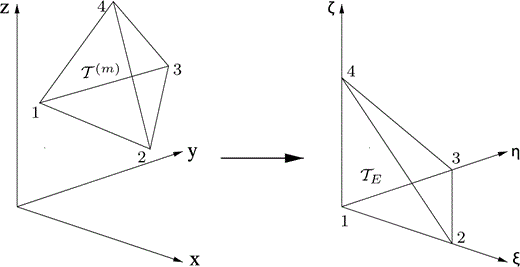
\includegraphics[width=0.6\linewidth]{figures/m_167-1-319-fig001.png}
    \caption{Transforming tetrahedron into a reference frame.(Figure taken from Figure 1 in ~\parencite{dumbser1})}
    \label{fig:transformation}
\end{figure}
As we are dealing with a new transformed coordinate system, we would need a Transformation matrix to transform the vector $Q_p$
from the global Cartesian system to the vector $Q_q^n$ in the normal, face-aligned frame. The transformation would be of the form

\begin{equation}
    Q_p = T_{pq}Q_q^n .
\end{equation}

\parencite{dumbser1} calculates the transformation matrix $T_{pq}$ as

\begin{align}
    \begin{split}
    T_{pq} = 
        \begin{bmatrix}
        n_x^2 & s_x^2 & t_x^2 & 2n_x s_x & 2s_x t_x & 2n_x t_x & 0 & 0 & 0 \\
        n_y^2 & s_y^2 & t_y^2 & 2n_y s_y & 2s_y t_y & 2n_y t_y & 0 & 0 & 0 \\
        n_z^2 & s_z^2 & t_z^2 & 2n_z s_z & 2s_z t_z & 2n_z t_z & 0 & 0 & 0 \\
        n_y n_x & s_y s_x & t_y t_x & n_y s_x + n_x s_y & s_y t_x + s_x t_y & n_y t_x + n_x t_y & 0 & 0 & 0 \\
        n_z n_y & s_z s_y & t_z t_y & n_z s_y + n_y s_z & s_z t_y + s_y t_z & n_z t_y + n_y t_z & 0 & 0 & 0 \\
        n_z n_x & s_z s_x & t_z t_x & n_z s_x + n_x s_z & s_z t_x + s_x t_z & n_z t_x + n_x t_z & 0 & 0 & 0 \\
        0 & 0 & 0 & 0 & 0 & 0 & n_x & s_x & t_x \\
        0 & 0 & 0 & 0 & 0 & 0 & n_y & s_y & t_y \\
        0 & 0 & 0 & 0 & 0 & 0 & n_z & s_z & t_z \\
    \end{bmatrix},
    \end{split}
\end{align}
where $\mathbf{n} = \left(n_x, n_y, n_z\right)^T$ are the components of the normal vector, and $\mathbf{s} = \left(s_x, s_y, s_z\right)^T$ and
$\mathbf{t} = \left(t_x, t_y, t_z\right)^T$ are the tangential vectors of the boundary face of the tetrahedron. $\mathbf{n}, \mathbf{s}, \mathbf{t}$
are orthogonal to each other. To represent the numerical solution $Q_h$ as a linear combination of pure spatial and pure time dependent functions, we introduce
the time-dependent degrees of freedom $\hat{Q}_m\left(t\right)$.

\begin{equation}
    Q_p^{\left(m\right)} \left(x,y,z,t\right) = \hat{Q}_{pl}^{\left(m\right)} \left(t\right) \Psi_l \left(x, y, z\right),
    \label{eq:mapping}
\end{equation}
where $\Psi_l\left(x,y,z\right)$ are spatial polynomial basis functions defined on the physical element. As it is more practical to define the polynomial 
basis functions on the reference element so that we can pre-calculate the integrals, we express equation \ref{eq:mapping} in 
the frame of the reference element using a suitable coordinate transformation M which maps the physical coordinates $\left(x, y, z\right)$ with the reference element $\left(\xi, \eta, \zeta\right)$

\begin{equation}
     Q_p^{\left(m\right)}\left(x,y,z,t\right) = \hat{Q}_{pl}^{\left(m\right)}\left(t\right) \Psi_l\left(M\left(x, y, z\right)\right).
\end{equation}

This formulation allows us to define the polynomial basis functions on the reference element $\Phi_l\left(\xi, \eta, \zeta\right)$.
As we can compute the integrals in the reference system beforehand, the coordinate transformation makes our implementation more computationally
efficient. This allows us to express $Q_h$ in each tetrahedron after the transformation of the coordinates
as 

\begin{equation}
    \left[Q_H^{\left(m\right)}\right]_p \left(\xi, \eta, \zeta, t\right) = \hat{Q}_{pl}^m \left(t\right) \Phi_l \left(\xi, \eta. \zeta\right),
\label{eq:solution}
\end{equation}
where $l$ denotes the $l^{th}$ basis function. Multiplying equation \ref{eq:compactform} with the test function $\Phi_k$ ~\parencite{cockburn2011discontinuous}
and integrating over our tetrahedral element $\mathcal{T}^{\left(m\right)}$ gives

\begin{equation}
    \int_{\mathcal{T}^{\left(m\right)}} \Phi_k \frac{\partial Q_p}{\partial t} dV + \int_{\mathcal{T}^{\left(m\right)}} \Phi_k \left(A_{pq} 
    \frac{\partial Q_q}{\partial x} + B_{pq}\frac{\partial Q_q}{\partial y} + C_{pq}\frac{\partial Q_q}{\partial z}\right)dV = 0.
    \label{eq:preweakformulation}
\end{equation}

We add fluxes $F_p^h$ at the boundaries of the tetrahedron to equation \ref{eq:preweakformulation} to include discontinuities in $Q_h$ and we integrate by parts to obtain the weak form as

\begin{equation}
    \int_{\mathcal{T}^{\left(m\right)}} \Phi_k \frac{\partial Q_p}{\partial t} dV + \int_{\partial \mathcal{T}^{\left(m\right)}} F_p^h dS
    - \int_{\mathcal{T}^{\left(m\right)}} \left(\frac{\partial \Phi_k}{\partial x} A_{pq}Q_q + \frac{\partial \Phi_k}{\partial y}B_{pq}Q_q
    + \frac{\partial \Phi_k}{\partial z}C_{pq}Q_q\right) dV = 0.
\label{eq:weakformulation}
\end{equation}

The flux between the tetrahedron $\mathcal{T}^{\left(m\right)}$ with the boundary extrapolated numerical solution $\hat{Q}_{sl} \Phi_l^{\left(m\right)}$
and one of its neighboring tetrahedra $\mathcal{T}^{\left(m_j\right)} \left(j=1,2,3,4\right)$ is computed in the global, coordinate system using the flux
matrix $A_{pq}$ from equation \ref{eq:fluxmatrix}

    \begin{align}
        \begin{split}
            F_p^h &= \frac{1}{2} T_{pq} \left(A_{qr}^{\left(m\right)} + \left|A_{qr}^{\left(m\right)}\right|\right)\left(T_{rs}\right)^{-1}
            \hat{Q}_{sl}^{\left(m\right)} \Phi_l^{\left(m\right)} \\
            &+ \frac{1}{2}T_{pq}\left(A_{qr}^{\left(m\right)} - \left|A_{qr}^{\left(m\right)}\right|\right)
            \left(T_{rs}\right)^{-1}\hat{Q}_{sl}^{\left(m_j\right)}\Phi_l^{\left(m_j\right)},            
        \end{split}
        \label{eq:fluxcalculation}
    \end{align}
where

\begin{equation}
\left|A_{qr}^{\left(m\right)}\right| = R_{qp}^A \left|\Lambda_{ps}\right| \left(R_{sr}\right)^{-1},
\end{equation}
and $\Lambda$ is the diagonal matrix with eigenvalues of $A_{pq}$ and $R_{pq}$ with right eigenvectors of $A_{pq}$ stacked in columns.
The next step would be inserting fluxes from equation \ref{eq:fluxcalculation} and $Q_h$ from equation \ref{eq:solution} into the weak
formulation in equation \ref{eq:weakformulation}. But as the basis functions $\Phi_l$ are defined in $\left(\xi, \eta, \zeta\right)$, we need
to transform the resulting equation with the transformation
\begin{equation}
    \text{d}x\, \text{d}y \, \text{d}z = \left|J\right| \text{d}\xi \,\text{d}\eta \,\text{d}\zeta,
\end{equation}
where $\left|J\right|$ is the determinant of the Jacobian matrix of the coordinate transformation and linear combination of the flux matrices to create transformed flux matrices
\begin{align}
    \begin{split}
        A_{pq}^{*} &= A_{pq} \frac{\partial \xi}{\partial x} + B_{pq} \frac{\partial \xi}{\partial y} + C_{pq} \frac{\partial \xi}{\partial z}, \\
        B_{pq}^{*} &= A_{pq} \frac{\partial \eta}{\partial x} + B_{pq} \frac{\partial \eta}{\partial y} + C_{pq} \frac{\partial \eta}{\partial z}, \\ 
        C_{pq}^{*} &= A_{pq} \frac{\partial \zeta}{\partial x} + B_{pq} \frac{\partial \zeta}{\partial y} + C_{pq} \frac{\partial \zeta}{\partial z}. 
    \end{split}
\end{align}

We finally get the semi-discrete \ac{DG} formulation of the ODE system within the reference tetrahedron $\mathcal{T}_E$
\begin{align}
    \begin{split}
        & \frac{\partial \hat{Q}_{pl}^{\left(m\right)}}{\partial t} \left|J\right| \int_{\mathcal{T}_E} \Phi_k \Phi_l d\xi d\eta d\zeta \\
        & + \sum_{j=1}^4 T_{pq}^j \frac{1}{2} \left(A_{qr}^{\left(m\right)} + \left| A_{qr}^{\left(m\right)}\right| \right) \left(T_{rs}^j\right)^{-1} \hat{Q}_{sl}^{\left(m\right)} \left|S_j\right| F_{kl}^{-,j} \\
        & + \sum_{j=1}^4 T_{pq}^j \frac{1}{2} \left(A_{qr}^{\left(m\right)} - \left| A_{qr}^{\left(m\right)}\right| \right) \left(T_{rs}^j\right)^{-1} \hat{Q}_{sl}^{\left(m_j\right)}\left|S_j\right| F_{kl}^{+,j,i,h} \\ 
        & - A_{pq}^* \hat{Q}_{ql}^{\left(m\right)} \left|J\right| \int_{\mathcal{T}_E} \frac{\partial \Phi_k}{\partial \xi} \Phi_l d\xi d\eta d\zeta \\
        & - B_{pq}^* \hat{Q}_{ql}^{\left(m\right)} \left|J\right| \int_{\mathcal{T}_E} \frac{\partial \Phi_k}{\partial \eta} \Phi_l d\xi d\eta d\zeta \\
        & - C_{pq}^* \hat{Q}_{ql}^{\left(m\right)} \left|J\right| \int_{\mathcal{T}_E} \frac{\partial \Phi_k}{\partial \zeta} \Phi_l d\xi d\eta d\zeta = 0,
    \end{split}
    \label{eq:finalform}
\end{align}
where 
\begin{align}
    \begin{split}
        F_{kl}^{-,j} &= \int_{\partial \left(\mathcal{T}_E\right)_j} \Phi_k \left(\xi^{\left(j\right)}\left(\chi, \tau\right)\right)\Phi_l \left(\xi^{\left(j\right)}\left(\chi, \tau\right)\right) d\chi d\tau, \quad \forall 1 \leq j\leq4 , \\
        F_{kl}^{+,j,i,h} &= \int_{\partial \left(\mathcal{T}_E\right)_j} \Phi_k \left(\xi^{\left(j\right)}\left(\chi, \tau\right)\right)\Phi_l \left(\xi^{\left(i\right)} \left( \tilde{\chi}^{(h)}\left(\chi, \tau\right), \tilde{\tau}^{\left(h\right)}\left(\chi, \tau\right) \right)\right) d\chi d\tau, \quad \forall 1 \leq i \leq 4, \quad 1 \leq h \leq 3.
    \end{split}
\end{align}

$F_{kl}^{-,j}$ accounts for the contribution of the element$\left(m\right)$ itself to the fluxes over face j and
$F_{kl}^{+,j,i,h}$ accounts for the contribution
of the element's direct side neighbor$\left(k_j\right)$ to the fluxes over the face $j$ and $\left|S_j\right|$ is the area of the face $j$ of the tetrahedron ~\parencite{dumbser1}. \\

\par We have not considered the source terms in the final formulation given in equation \ref{eq:finalform}. The source terms are dealt with as presented in~\parencite{10.1785/0120060253}.

\subsection[ADER Time Discretization]{ADER Time Discretization}

Instead of now utilizing the Runge-Kutta method to derive a limited fourth-order in time Runge-Kutta \ac{DG} scheme, we adopt the 
\ac{ADER} approach to achieve an arbitrary high-order accuracy in both spatial and temporal dimensions. Runge-Kutta schemes of order
higher than 4 tend to become inefficient as the number of calculation steps required exceeds the order of accuracy due to the Butcher barriers~\parencite{butcher1987numerical}.

\par By applying the \ac{ADER} scheme to the \ac{DG} formulation described in equation \ref{eq:finalform}, we obtain the \ac{ADER}-\ac{DG} scheme.
The crucial step in this approach involves using the Cauchy-Kovalewski procedure to replace time-derivatives with pure space derivatives.
As a consequence, the Cauchy-Kovalewski procedure provides the $k^{th}$ time-derivative as shown in equation \ref{eq:cauchy-kovalewski} in the face-aligned coordinate system, allowing us to
achieve higher accuracy without the limitations of tradiational Runge-Kutta schemes

\begin{equation}
    \frac{\partial^k Q_p}{\partial t^k} = \left(-1\right)^k \left(A_{pq}^* \frac{\partial}{\partial \xi} + B_{pq}^* \frac{\partial}{\partial \eta} + C_{pq}^* \frac{\partial}{\partial \zeta}\right)^k Q_q .
    \label{eq:cauchy-kovalewski}
\end{equation}

$Q_p$ can be expanded in a Taylor series with respect to time, and then the time derivatives can be substituted with space derivatives
using the equation \ref{eq:cauchy-kovalewski}~\parencite[Sec. 3.2]{dumbser1}. By adopting this approach, we can achieve arbitrary high-order
accuracy in both spatial and temporal dimensions. As previously mentioned, the \ac{ADER}-\ac{DG} schemes conduct time integration
within a single time step, considering only the current element and its neighboring elements, making it well-suited for parallelization.
Moreover, studies have demonstrated that the \ac{ADER}-\ac{DG} method outperforms traditional schemes such as \ac{RK-DG} scheme ~\parencite{dumbser2005ader}.
\subsection{Boundary Conditions}
Up until now, we have explored the time-discretization and space-discretization aspects of our problem. To complete our numerical
solver, we must establish suitable boundary conditions for the problem. We mainly have three kinds of boundaries in consideration.
\subsubsection{Absorbing Boundaries}
With the implementation of absorbing boundary conditions, the physical volume is enclosed by such boundaries in the forward direction. This means that no waves enter the computational domain, and any outgoing waves smoothly pass through the boundary without experiencing
reflection. A careful examination of equation \ref{eq:fluxcalculation} reveals that its first term on the right-hand side corresponds
to the outflow from the current element, while the second term represents the inflow from neighboring elements. To prevent incoming
waves from affecting the solution, we set the second term to zero. Consequently, the flux at all absorbing faces of the respective
tetrahedral elements is then appropriately set to

\begin{equation}
    F_p^{AbsorbBC} = \frac{1}{2} T_{pq} \left(A_{qr}^{\left(m\right)} + \left|A_{qr}^{\left(m\right)}\right|\right) \left(T_{rs}\right)^{-1} \hat{Q}_{sl}^{\left(m\right)} \Phi_l^{\left(m\right)}.
\end{equation}

\subsubsection{Free-Surface Boundaries}
At a free-surface boundary, the elastic medium is in contact with the surrounding air or void. In this scenario, there are no external forces
acting on the outside of the elastic medium. To ensure that normal and shear stresses vanish at the free surface, a technique involving
ghost cells is employed. These ghost cells are used to mirror the stresses, such that their values have the same magnitude as the actual
stresses but with the opposite sign. This approach effectively satisfies the condition of stress equilibrium at the free surface, allowing
for an accurate treatment at the boundary. We implement this using the flux function ~\parencite{dumbser1}

\begin{align}
    \begin{split}
    F_{p}^{FreeBC} &= \frac{1}{2}T_{pq}\left(A_{qr}^{\left(m\right)} + \left|A_{qr}^{\left(m\right)}\right|\right) \left(T_{rs}\right)^{-1} \hat{Q}_{sl}^{\left(m\right)} \Phi_l^{\left(m\right)}
    \\ &+ \frac{1}{2} T_{pq} \left(A_{qr}^{\left(m\right)} - \left|A_{qr}^{\left(m\right)}\right|\right) \Gamma_{rs} \left(T_{st}\right)^{-1} \hat{Q}_{tl}^{\left(m\right)} \Phi_l^{\left(m\right)} ,
    \end{split}
\end{align}
where $\Gamma_{rs} = diag\left(-1,1,1,-1,1,-1,1,1,1\right)$ is the matrix which mirrors the normal and shear stresses.

\section{Summary}
In this chapter we have discussed the governing equations of linear elasticity as a sytem of hyperbolic \ac{PDE}s. We then discussed the 
\ac{ADER}-\ac{DG} method for numerically solving this system of equations. We have also looked at the boundary conditions that we will use in our numerical solver.

\chapter{Time Reversal}\label{chapter:TimeReversal}

Time-reversal methods involve mirroring the propagation of waves in time, aiming to converge the resulting wave back to its source.~\parencite{Fink2017} mentions two ways to achieve time-reversal.
The first method involves \ac{TRM}s, which rely on Cauchy boundary conditions. If the wavefield and its normal derivative are known at the entire surface $S$ surrounding the volume
$V$ at all times $t$, the wavefield inside the entire volume can be computed. In this approach, the outgoing wave is initially 
recorded on $S$, then time-reversed and finally emitted from $S$. \\

Alternatively, time-reversal can be achieved with manipulation of the initial conditions. In this case, the wavefield and its normal derivative
are known inside the entire volume but only for a specific time. 
~\parencite{Weinert2016} describes Loschmidt's demon as something hypothetical which reverses the momentum/velocity of each particle instantaneously such that the state of the system is reversed 
from a fibrillated state to a less fibrillated, smoother state.
By doing something which mimicks Loschmidt's demons ~\parencite{Weinert2016}, ~\parencite{Fink2017} which act simultaneously on the entire space, the velocity of each particle can be instantaneously reversed, resulting in a time-reversed wave. This approach is known as the \ac{ITM}.\\

This thesis primarily focuses on the \ac{ITM} approach for seismic waves. In this method, a time-reversed wave is generated through a sudden modification of the wave propagation
properties of the medium~\parencite{Bacot2016}. Section \ref{section:ITMTheory} delves into the theoretical foundation behind the \ac{ITM}, providing a comprehensive
understanding of its principles. In the latter part of the chapter, we present the implementation of \ac{ITM} within the numerical simulation software SeisSol. The
description of the implementation is kept as general as possible, allowing for a broad grasp of the method's application and utility.

\section{Theory of Instantaneous Time Mirrors}\label{section:ITMTheory}

Time-reversal methods for waves are based on the time-reversal invariance of wave equations. They rely on the fact that any wave-field can be completely determined within
a volume by knowing the field(and its normal derivative) on any enclosing surface~\parencite{Bacot2016}. We write the elastic wave equation in its second order vector form
~\parencite[Cha. 2]{aki2002quantitative} as
\begin{equation}
    \rho \ddot{\mathbf{U}} \left( \mathbf{x}, t\right) - \left( \lambda + 2 \mu \right) \nabla \left(\nabla \cdot \mathbf{U}\left(\mathbf{x}. t\right)\right) 
    + \mu \nabla \times \left(\nabla \times \mathbf{U}\left(\mathbf{x},t\right)\right) = \mathbf{S}\left(\mathbf{x},t\right),
\end{equation}

with the source function $\mathbf{S}\left(\mathbf{x},t\right)$ contains only second order time derivatives. This implies that if $\hat{\mathbf{U}}\left(\mathbf{x},t\right)$
is a solution, then $\hat{\mathbf{U}}\left(\mathbf{x}, -t\right)$ is also a solution, if $\mathbf{S}$ is symmetric in time such that 
$\mathbf{S}\left(\mathbf{x}, t\right) = \mathbf{S}\left(\mathbf{x}, -t\right)$. \\

The \ac{ITM} approach is closely connected to the Cauchy theorem, which states that the wave field evolution can be deduced from the knowledge of thie wave field
and its derivative at one single time, i.e., the initial conditions. By inducing a sudden modification of the wave propagation properties(such as impedance) in the
medium, a time-reversed wave is generated. This modification, referred to as the \ac{ITM}, does not require the use of antennas or the entire wave field's memory~\parencite{Bacot2016}.
~\parencite{Bacot2016} demonstrated this for water waves with physical and numerical experiments resulting in successful refocusing of the generated waves into their
sources' shapes. This was achieved by introducing a temporal slab in the wave velocities like in figure \ref{fig:deltavelocity}

\begin{figure}
    \centering
    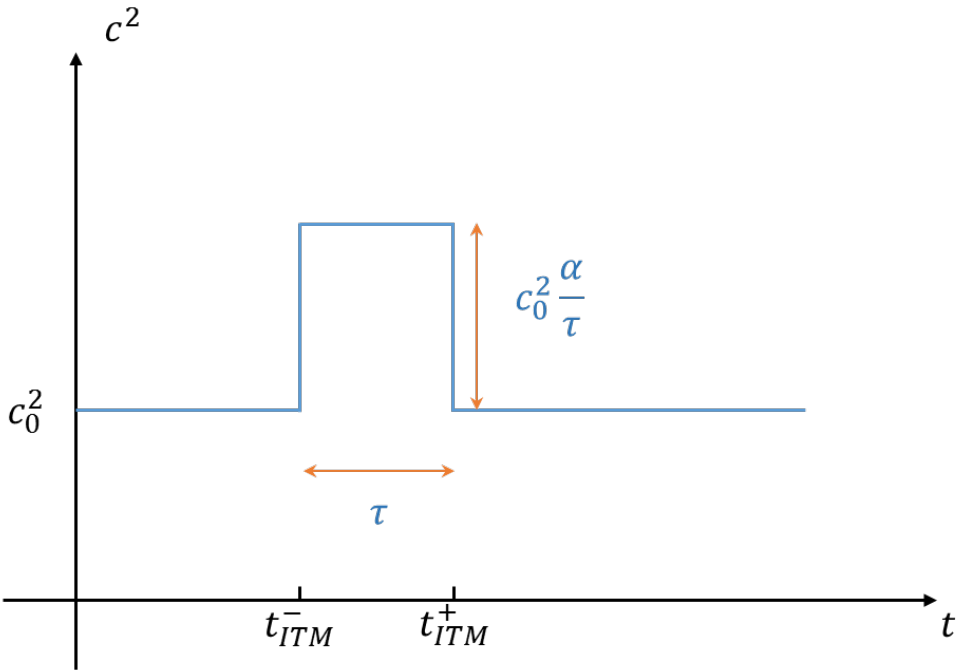
\includegraphics[width=0.6\linewidth]{figures/delta_speed.png}
    \caption{Rectangular profile for the wave velocity.(Figure taken from Figure 1 in ~\parencite[Supplementary Material]{Bacot2016})}
    \label{fig:deltavelocity}
\end{figure}

In the context of elastic waves, as we have seen in equations \ref{eq:setofequations} and \ref{eq:wavevelocities}, there are two propagating waves, i.e., P- and S- waves. 
~\parencite[Sec 9.6-Sec 9.8]{leveque_2002} shows that in case of spacial material interfaces, a discontinuity in the quantity called Impedance $Z = \rho v$
causes reflections across the material interface. ~\parencite[Eq. 1.66 and 1.180]{kaufman} show that impedances of P- and S- waves are defined analogously as
$Z_p = \rho v_p$ and $Z_s = \rho v_s$.
% !TeX root = ../main.tex
% Add the above to each chapter to make compiling the PDF easier in some editors.
\section{\texorpdfstring{\ac{ITM} on a one-dimensional acoustic planar wave}{ITM on a one-dimensional acoustic planar wave}}\label{section:ITMAcoustic}
In this section, we calculate the analytical solution for a one-dimensional acoustic wave when an \ac{ITM} is applied from $t_{ITM}^-$ to $t_{ITM}^+$.
For this, we consider a one-dimensional acoustic equation ~\parencite[Sec. 2.8]{leveque_2002} linearized about the motionless state
\begin{align}
    \begin{split}
        p_t + K_0u_x = 0, \\
        u_t + \frac{1}{\rho_0}p_x = 0 ,\\
    \end{split}
\end{align}
where $p$ is the pressure perturbation, $K_0$ is the bulk modulus of the material and $u$ is the velocity perturbation. 
This can be written in consolidated matrix vector form as done for first order hyperbolic systems of equations as follows
\begin{align}
    \begin{split}
        \frac{\partial }{\partial t}
    \begin{bmatrix}
        p \\
        u
    \end{bmatrix} + 
    \begin{bmatrix}
        0 & K_0 \\
        \frac{1}{\rho_0} & 0 \\
    \end{bmatrix}
    \frac{\partial }{\partial x}
    \begin{bmatrix}
        p \\
        u
    \end{bmatrix} = 0 .
    \end{split}
    \label{eq:acoustic}
\end{align}

The flux matrix of equation \ref{eq:acoustic} has two eigenvalues
\begin{align}
    \begin{split}
        \lambda_1 = -c_0, \quad \lambda_2 = c_0,
    \end{split}
\end{align}
where 
\begin{align}
    \begin{split}
        c_0 = \sqrt{\frac{K_0}{\rho_0}}
    \end{split}
\end{align}
is the speed of sound. Waves can propagate in either direction with this speed. The eigenvectors for this coefficient matrix are
\begin{align}
    \begin{split}
        r^1 = \begin{bmatrix}
            -\rho_0 c_0 \\
            1
        \end{bmatrix}, \quad
        r^2 = \begin{bmatrix}
            \rho_0 c_0 \\
            1
        \end{bmatrix}.
    \end{split}
\end{align}

The impedance as mentioned in section \ref{section:ITMTheory} is defined as
\begin{equation}
    Z_0 = \rho_0 c_0.
\end{equation}
\par Using these parameters, ~\parencite[Sec. 2.8]{leveque_2002} calculates the solution of the acoustic equation depending on the initial conditions $p^0(x), u^0(x)$ as:
\begin{align}
    \begin{split}
        p(x,t) &= \frac{1}{2}\left[p^0\left(x + c_0t\right) + p^0\left(x - c_0t\right)\right] - \frac{Z_0}{2}\left[u^0\left(x+c_0t\right) - u^0\left(x-c_0t\right)\right], \\
        u(x,t) &= -\frac{1}{2Z_0}\left[p^0\left(x+c_0t\right) - p^0\left(x-c_0t\right)\right] + \frac{1}{2}\left[u^0\left(x+c_0t\right) + u^0\left(x-c_0t\right)\right] .
    \end{split}
    \label{eq:solutionacoustic}
\end{align}

We use this solution to find the analytical solution of a 1D acoustic wave after the \ac{ITM} is applied in two different ways. First we ensure we use initial conditions which give rise to only one forward wave. We simply use a sinusoidal wave multiplied with one eigenvector $r^2$.
This defines our initial conditions as
\begin{align}
    \begin{split}
        p^0\left(x\right) &= \rho_0c_0 \cos\left(kx\right), \\
        u^0\left(x\right) &= \cos\left(kx\right) ,
    \end{split}
    \label{eq:initialconditions}
\end{align}
where $k$ is the wave number of the wave. To ensure that our domain is periodic, we defined our domain to be between two wavelengths, i.e., from 
$\left[-\frac{\pi}{k}, \frac{\pi}{k}\right]$. The energy of the system is defined in this domain as ~\parencite{Kopriva2021}

\begin{equation}
     E_1 = \int_{-\frac{\pi}{k}}^{\frac{\pi}{k}} \left(\frac{1}{2K}p^2 + \frac{1}{2}\rho u^2\right) dx,
    \label{eq:energy}
\end{equation}
which simplifies to
\begin{equation}
    E_1 = \frac{\pi\rho_0}{k},
\end{equation}
for phase 1. Energy defined in equation \ref{eq:energy} is conserved for a particular phase as the system of equations are conservative for every phase ~\parencite{Kopriva2021}. 

\subsection{\texorpdfstring{Impedance Changing \ac{ITM}}{Impedance Changing ITM}}\label{section:impedancechangingITM}
Using the conditions given by equation \ref{eq:initialconditions}, we calculate the solution at $t_{ITM}^-$ and use them as initial conditions for the new equation where the material properties are changed.
In this case, we modify the material properties such that the velocities are scaled while the impedance also changes. This is achieved by modifying the bulk modulus while keeping the density constant. Using \ref{eq:solutionacoustic}, we get the initial conditions for the next phase of the simulation$\left(t_{ITM}^- \leq t \leq t_{ITM}^+ \right)$ at $t_{ITM}^-$ as
\begin{align}
    \begin{split}
        p^0_{t_{ITM}^-}\left(x\right) &= c_0 \rho_0 \cos\left(kx - c_0kt_{ITM}^-\right), \\
        u^0_{t_{ITM}^-}\left(x\right) &= \cos\left(kx - c_0kt_{ITM}^-\right) .
    \end{split}
\end{align}

We now use these initial conditions and equation \ref{eq:solutionacoustic} with the updated wave velocity and constant density to get the evolved solution for $t_{ITM}^- \leq t \leq t_{ITM}^+ $. We used~\parencite{sagemath} to perform the arithmetic simplifications. We obtain the solution for this period as
\begin{align}
    \begin{split}
        p_{2}\left(x, t\right) &= -\frac{1}{2} \left(n-1\right)c_0\rho_0 \cos\left(kx + c_0knt - \left(c_0kn + c_0k\right)t_{ITM}^-\right) \\
        &+ \frac{1}{2} \left(n+1\right)c_0\rho_0\cos\left(kx - c_0knt + \left(c_0kn - c_0k\right)t_{ITM}^-\right), \\
        u_{2}\left(x, t\right) &= \frac{1}{2}\left(n-1\right)\cos\left(kx + c_0knt - \left(c_0kn + c_0k\right)t_{ITM}^-\right)\\
        &+ \frac{1}{2}\left(n+1\right)\cos\left(kx - c_0knt + \left(c_0kn-c_0k\right)t_{ITM}^-\right) ,
    \end{split}
\end{align}
where n is the velocity scaling factor. We now use these expressions to calculate the energy as we have already done in equation \ref{eq:energy}. This gives us the energy in the second phase, i.e., $t_{ITM}^- \leq t \leq t_{ITM}^+ $ to be
\begin{equation}
    E_2 = \frac{1}{2}\frac{\left(1 + n^2\right)\pi \rho_0}{kn^2} .
\end{equation}

This shows that the energy drops when the velocity is scaled up. We then check the relative drop in energy for different scaling factors and see that it asymptotes to 0.5 for higher scaling factors. The variation of the ratio with the scaling factor can be seen in figure \ref{fig:ratio1}.

\begin{figure}[!htpb]
    \centering
    \begin{tikzpicture}[scale=1.0]
        \begin{axis}[
            ylabel = $\frac{E_2}{E_1}$,
            xlabel = $n$]
            \addplot[domain=0:10, black, ultra thick]{0.5*(1+x*x)/(x*x)};
            \addplot[domain=0:10, black, ultra thick, densely dotted]{0.5};
        \end{axis}
    \end{tikzpicture}
    \caption{Relative Energy $\left(\frac{E_2}{E_1}\right)$ in $t_{ITM}^- \leq t \leq t_{ITM}^+$. }
    \label{fig:ratio1}
\end{figure}

Now, the velocity is scaled back to its initial value at $t=t_{ITM}^+$. By defining $\tau = t_{ITM}^+ - t_{ITM}^-$, a similar calculation is performed to acquire the
solution for the final phase, i.e., $t \geq t_{ITM}^+$, and the resulting solution is
\begingroup
\allowdisplaybreaks
\begin{align}
    \begin{split}
        p_3\left(x, t\right) & = -\frac{{\frac{1}{4}c_{0}\rho_{0}\left( -n^{2} + 1\right)} \cos\left(k x + c_{0} k t - 2 \, c_{0} k \mathit{t_{ITM}^-} - {\left(c_{0} k n + c_{0} k\right)} \tau\right)}{n} \\
        & - \frac{{\frac{1}{4}c_0\rho_0\left(n^{2} - 1\right)} \cos\left(k x + c_{0} k t - 2 \, c_{0} k \mathit{t_{ITM}^-} + {\left(c_{0} k n - c_{0} k\right)} \tau\right)}{n} \\
        & - \frac{{\frac{1}{4}c_0\rho_0\left(n^{2} - 2n + 1\right)} \cos\left(kx -c_{0} k t + {\left(c_{0} k n + c_{0} k\right)} \tau\right)}{n} \\
        & - \frac{{\frac{1}{4}c_0\rho_0\left(-n^{2} - 2n - 1\right)} \cos\left(kx-c_{0} k t - {\left(c_{0} k n - c_{0} k\right)} \tau\right)}{n}, \\
        u_3\left(x, t\right) & =  -\frac{{\frac{1}{4}\left(n^{2} - 1\right)} \cos\left( k x + c_{0} k t - 2 \, c_{0} k \mathit{t_{ITM}^-} - {\left(c_{0} k n + c_{0} k\right)} \tau\right)}{n} \\
        & - \frac{{\frac{1}{4}\left(-n^{2} + 1\right)} \cos\left(kx + c_{0} k t - 2 \, c_{0} k \mathit{t_{ITM}^-} + {\left(c_{0} k n - c_{0} k\right)} \tau\right)}{n} \\
        & - \frac{{\frac{1}{4}\left(n^{2} - 2n + 1\right)} \cos\left(kx -c_{0} k t + {\left(c_{0} k n + c_{0} k\right)} \tau\right)}{n} \\
        & - \frac{{\frac{1}{4}\left(-n^{2} - 2n - 1\right)} \cos\left(kx -c_{0} k t - {\left(c_{0} k n - c_{0} k\right)} \tau\right)}{n} .
    \end{split}
\end{align}
\endgroup

Using these quantities, we now calculate the energy using the equation \ref{eq:energy}
\begin{equation}
    E_3 = -\pi \rho_0\frac{{\left(1 + n^{4} - 2 \, n^{2}\right)} \cos^{2}\left(c_{0} k n \tau\right) - {\left(1 + n^{4}\right)}}{2 \, k n^{2}}.
\end{equation}

The final energy $E_3$ is dependent on the parameters: $k, n, \tau$ and is bounded as

\begin{equation}
    \frac{\pi \rho_0}{K} \leq E_3 \leq \frac{\pi \rho_0}{2K}\left[n^2 + \frac{1}{n^2}\right] .
\end{equation}

This demonstrates that the application of \ac{ITM} leads to a change in the energy of our system. We compare the worst case scenario, i.e., what would be the maximum energy increase after the ITM is applied. For that,
 we take the upper bound and plot the ratio $\frac{E_3}{E_1}$ with $n$ as we did before in figure \ref{fig:ratio2}.

\begin{figure}[!htpb]
    \centering
    \begin{tikzpicture}[scale=1.0]
        \begin{axis}[
            ylabel = $\frac{E_3}{E_1}$,
            xlabel = $n$]
            \addplot[domain=0.1:10, samples=1001, black, ultra thick]{0.5*((1/x)^2 + x^2)};
        \end{axis}
    \end{tikzpicture}
    \caption{Maximum Relative Energy$\left(\frac{E_3}{E_1}\right)$ in $t \geq t_{ITM}^+$}
    \label{fig:ratio2}
\end{figure}

The minimum value for this energy jump lies at $n=1$, which means no velocity scaling and no reflections. This particular scenario does not offer any practical utility
or relevance to our objective.

\subsection{\texorpdfstring{Constant Impedance \ac{ITM}}{Constant Impedance ITM}}
We know that there is no reflected wave in space interfaces when the impedance stays constant~\parencite[Sec 9.7]{leveque_2002}. Here, we test out the same with a time interface, i.e., we perform \ac{ITM} such that the velocities scale but the impedance stays constant. This is achieved by scaling the wave speed by $n$ and the density by $\frac{1}{n}$.
Similar to section \ref{section:impedancechangingITM}, we choose the initial conditions as
\begin{align}
    \begin{split}
        p^0\left(x\right) &= Z_0 \cos\left(kx\right), \\
        u^0\left(x\right) &= \cos\left(kx\right) .
    \end{split}
    \label{eq:initialconditions2}
\end{align}

Using these parameters, the energy is once again computed as in equation \ref{eq:energy} and is found to be
\begin{equation}
    E_1 = \frac{\pi Z_0}{c_0 k} .
\end{equation}

Using the conditions given in equation \ref{eq:initialconditions2}, we calculate the solution at $t_{ITM}^-$ and use them as initial conditions for the new equation where the wave velocities are scaled.
In this case, we scale the velocities such that the impedance does not change. This is achieved by scaling the density down. Using \ref{eq:solutionacoustic}, we get the initial conditions for the next phase of the simulation$\left(t_{ITM}^- \leq t \leq t_{ITM}^+ \right)$ at $t_{ITM}^-$ as
\begin{align}
    \begin{split}
        p^0_{t_{ITM}^-}\left(x\right) &= Z_0 \cos\left(kx - c_0kt_{ITM}^-\right), \\
        u^0_{t_{ITM}^-}\left(x\right) &= \cos\left(kx - c_0kt_{ITM}^-\right) .
    \end{split}
\end{align}

We now use these as the initial conditions and equation \ref{eq:solutionacoustic} with the updated wave velocity and constant density to get the evolved solution for $t_{ITM}^- \leq t \leq t_{ITM}^+ $. 
We used ~\parencite{sagemath} to perform the simplifications for the arithmetic. We obtain the solution for this period as
\begin{align}
    \begin{split}
        p_{2}\left(x, t\right) &= Z_{0} \cos\left(kx -c_{0} k n t + {\left(c_{0} k n - c_{0} k\right)} \mathit{t_{ITM}^-}\right), \\
        u_{2}\left(x, t\right) &= \cos\left(kx -c_{0} k n t + {\left(c_{0} k n - c_{0} k\right)} \mathit{t_{ITM}^-} \right) ,
    \end{split}
\end{align}
where n is the velocity scaling factor. We now use these expressions to calculate the energy using equation \ref{eq:energy}. This gives us the energy in the second phase, i.e., $t_{ITM}^- \leq t \leq t_{ITM}^+ $ to be
\begin{equation}
    E_2 = \frac{\pi z_{0}}{c_{0} k n} .
\end{equation}

We obverse that there is no extra reflected wave and the wave speed is just increased with a phase shift and that the energy is directly scaled down by the velocity scaling factor.

% \begin{figure}
%     \centering
%     \begin{tikzpicture}[scale=1.0]
%         \begin{axis}[
%             ylabel = $\frac{E_2}{E_1}$,
%             xlabel = $n$]
%             \addplot[domain=0:10, black, ultra thick]{0.5*(1+x*x)/(x*x)};
%         \end{axis}
%     \end{tikzpicture}
%     \caption{Relative Energy in $t_{ITM}^- \leq t \leq t_{ITM}^+$}
%     \label{fig:ratio1}
% \end{figure}

Now, the velocity is scaled down again to its original value at $t=t_{ITM}^+$ and defining $\tau = t_{ITM}^+ - t_{ITM}^-$, we do a similar calculation to obtain the solution for the final phase, i.e., $t \geq t_{ITM}^+$ as
\begin{align}
    \begin{split}
        p_3\left(x, t\right) & = Z_{0} \cos\left(kx - c_{0} k t - {\left(c_{0} k n - c_{0} k\right)} \tau\right) , \\
        u_3\left(x, t\right) & =  \cos\left(kx - c_{0} k t - {\left(c_{0} k n - c_{0} k\right)} \tau\right) . 
    \end{split}
\end{align}

Using these quantities, we now calculate the energy using equation \ref{eq:energy}
\begin{equation}
    E_3 = \frac{\pi Z_0}{c_0 k} ,
\end{equation}
which is equal to $E_1$. This shows that there is no final energy increase when the impedance is kept constant. The final solution also has no reflected wave and has the same wave speed as the initial wave and has a phase shift in time. This confirms that even in time interfaces, similar to space interfaces there is no reflection.

% \begin{align}
%     \begin{split}
%         \left(\left(\begin{array}{rrrr}
%             1 & 1 & 0 & 0 \\
%             -\frac{k_{1}}{\rho_{0} \sqrt{\frac{K_{0} k_{1}^{2} + K_{0} k_{2}^{2} + K_{0} k_{3}^{2}}{\rho_{0}}}} & \frac{k_{1}}{\rho_{0} \sqrt{\frac{K_{0} k_{1}^{2} + K_{0} k_{2}^{2} + K_{0} k_{3}^{2}}{\rho_{0}}}} & 1 & 0 \\
%             -\frac{k_{2}}{\rho_{0} \sqrt{\frac{K_{0} k_{1}^{2} + K_{0} k_{2}^{2} + K_{0} k_{3}^{2}}{\rho_{0}}}} & \frac{k_{2}}{\rho_{0} \sqrt{\frac{K_{0} k_{1}^{2} + K_{0} k_{2}^{2} + K_{0} k_{3}^{2}}{\rho_{0}}}} & 0 & 1 \\
%             -\frac{k_{3}}{\rho_{0} \sqrt{\frac{K_{0} k_{1}^{2} + K_{0} k_{2}^{2} + K_{0} k_{3}^{2}}{\rho_{0}}}} & \frac{k_{3}}{\rho_{0} \sqrt{\frac{K_{0} k_{1}^{2} + K_{0} k_{2}^{2} + K_{0} k_{3}^{2}}{\rho_{0}}}} & -\frac{k_{1}}{k_{3}} & -\frac{k_{2}}{k_{3}}
%             \end{array}\right)\right)
%     \end{split}
% \end{align}

\section{\texorpdfstring{\ac{ITM}}{ITM} on a 3D acoustic planar wave}\label{section:3DITMAcoustic}
In this section, we calculate the analytical solution for a 3D Acoustic wave when an \ac{ITM} is applied from $t_{ITM}^-$ to $t_{ITM}^+$.

To do this, we consider a three dimensional acoustic equation linearised over the stationary state, where $p$ is the pressure perturbation, $K_0$ is the bulk
modulus of the material and $u,\,v,\,w$ are the velocity perturbations in $x,\,y,\,z$ respectively. This can be written in consolidated matrix vector form as done for first order hyperbolic systems of equations as

\begin{align}
    \begin{split}
        \frac{\partial}{\partial t}\mathbf{q} + \mathbf{A}\frac{\partial}{\partial x}\mathbf{q} + \mathbf{B}\frac{\partial}{\partial y}\mathbf{q} + 
        \mathbf{C}\frac{\partial}{\partial z}\mathbf{q} = 0,
    \end{split}
    \label{eq:3Dacoustic}
\end{align}
where
\begin{align}
    \begin{split}
        \mathbf{q} = \begin{bmatrix}
            p \\
            u \\
            v \\
            w 
        \end{bmatrix}, \quad
        \mathbf{A} = \begin{bmatrix}
            0 & K_0 & 0 & 0 \\
            \frac{1}{\rho_0} & 0 & 0 & 0 \\
            0 & 0 & 0 & 0 \\
            0 & 0 & 0 & 0 \\
        \end{bmatrix}, \quad
        \mathbf{B} = \begin{bmatrix}
            0 & 0 & K_0 & 0 \\
            0 & 0 & 0 & 0 \\
            \frac{1}{\rho_0} & 0 & 0 & 0 \\
            0 & 0 & 0 & 0 \\
        \end{bmatrix}, \quad
        \mathbf{C} = \begin{bmatrix}
            0 & 0 & 0 & K_0 \\
            0 & 0 & 0 & 0 \\
            0 & 0 & 0 & 0 \\
            \frac{1}{\rho_0} & 0 & 0 & 0 \\
        \end{bmatrix} \quad .
    \end{split}
\end{align}

We assume an ansatz of 
\begin{equation}
    \mathbf{q}\left(\mathbf{x}, t\right) = \mathbf{q_0} \cos\left(\mathbf{k}\cdot\mathbf{x} - \omega t\right),
\end{equation}
where $\mathbf{k}=\left(k_1, k_2, k_3\right)$ is the wave number of the planar wave. Using the derivatives of equation \ref{eq:3Dacoustic},
\begin{align}
    \begin{split}
    \frac{\partial \mathbf{q}}{\partial t} &= \omega \mathbf{q_0} \sin\left(\mathbf{k}\cdot\mathbf{x} - \omega t\right), \\
    \frac{\partial \mathbf{q}}{\partial x} &= -k_1 \mathbf{q_0} \sin\left(\mathbf{k}\cdot\mathbf{x} - \omega t\right), \\
    \frac{\partial \mathbf{q}}{\partial y} &= -k_2 \mathbf{q_0} \sin\left(\mathbf{k}\cdot\mathbf{x} - \omega t\right), \\
    \frac{\partial \mathbf{q}}{\partial z} &= -k_3 \mathbf{q_0} \sin\left(\mathbf{k}\cdot\mathbf{x} - \omega t\right).
\end{split}
\end{align}

Substituting these back in the equation we get
\begin{align}
    \begin{split}
        \left(\omega - \mathbf{A}k_1 - \mathbf{B}k_2 - \mathbf{C}k_3\right)\mathbf{q_0}\sin\left(\mathbf{k}\cdot\mathbf{x} - \omega t\right) = 0.
    \end{split}
\end{align}

Dividing by $\sin\left(\mathbf{k}\cdot\mathbf{x} - \omega t\right)$ and rearranging the terms, we get
\begin{align}
    \begin{split}
        \left(\mathbf{A}k_1 + \mathbf{B}k_2 + \mathbf{C}k_3\right)\mathbf{q_0} = \omega \mathbf{q_0} .
    \end{split}
\end{align}

This shows that $\omega$ is an eigenvalue of $\mathbf{\hat{A}} = \mathbf{A}k_1 + \mathbf{B}k_2 + \mathbf{C}k_3$ and $\mathbf{q_0}$ is an eigenvector. The modified matrix $\mathbf{\hat{A}}$ would then be
\begin{align}
    \begin{split}
    \mathbf{\hat{A}} = \left(\begin{array}{rrrr}
0 & K_{0} k_{1} & K_{0} k_{2} & K_{0} k_{3} \\
\frac{k_{1}}{\rho_{0}} & 0 & 0 & 0 \\
\frac{k_{2}}{\rho_{0}} & 0 & 0 & 0 \\
\frac{k_{3}}{\rho_{0}} & 0 & 0 & 0
\end{array}\right) ,
    \end{split}
\end{align}
with the set of eigenvalues after replacing $\sqrt{\frac{K_{0}}{\rho_{0}}}$ with $c$
\begin{align}
    \begin{split}
        \omega_1 = -c \sqrt{k_{1}^{2} + k_{2}^{2} + k_{3}^{2}}, \quad
        \omega_2 = 0, \quad
        \omega_3 = 0, \quad 
        \omega_4 = c \sqrt{k_{1}^{2} + k_{2}^{2} + k_{3}^{2}},
    \end{split}
\end{align}
and the eigenvectors after replacing $\rho_0 \sqrt{\frac{K_0}{\rho_0}}$ with $Z_0$,
\begin{align}
    \begin{split}
    \mathbf{r_1} = \begin{bmatrix}
        1 \\
-\frac{k_{1}}{Z_0 \sqrt{k_{1}^{2} + k_{2}^{2} + k_{3}^{2}}} \\
-\frac{k_{2}}{Z_0 \sqrt{k_{1}^{2} + k_{2}^{2} + k_{3}^{2}}} \\
-\frac{k_{3}}{Z_0 \sqrt{k_{1}^{2} + k_{2}^{2} + k_{3}^{2}}}
        \end{bmatrix}, \quad
        \mathbf{r_2} = \begin{bmatrix}
            0 \\
1 \\
0 \\
-\frac{k_{1}}{k_{3}}
            \end{bmatrix}, \quad
            \mathbf{r_3} = \begin{bmatrix}
                0 \\
                0 \\
                1 \\
                -\frac{k_{2}}{k_{3}}
                \end{bmatrix}, \quad
                \mathbf{r_4} = \begin{bmatrix}
                    1 \\
\frac{k_{1}}{Z_0 \sqrt{k_{1}^{2} + k_{2}^{2} + k_{3}^{2}}} \\
\frac{k_{2}}{Z_0 \sqrt{k_{1}^{2} + k_{2}^{2} + k_{3}^{2}}} \\
\frac{k_{3}}{Z_0 \sqrt{k_{1}^{2} + k_{2}^{2} + k_{3}^{2}}}
                    \end{bmatrix} .
    \end{split}
\end{align}

For the sake of simplicity, we choose $\left(k_1,k_2,k_3\right) = \left(k,0,0\right)$ inducing our wave to travelling along the x-axis. This makes our eigenvalues
\begin{align}
    \begin{split}
        \omega_1 = -k c, \quad
        \omega_2 = 0, \quad
        \omega_3 = 0, \quad
        \omega_4 = k c .
    \end{split}
\end{align}

We get our eigenvectors as
\begin{align}
    \begin{split}
    \mathbf{r_1} = \begin{bmatrix}
        1 \\
-\frac{1}{Z_0} \\
0 \\
0
        \end{bmatrix}, \quad
        \mathbf{r_2} = \begin{bmatrix}
            0 \\
0 \\
0 \\
1
            \end{bmatrix}, \quad
            \mathbf{r_3} = \begin{bmatrix}
                0 \\
                0 \\
                1 \\
                0
                \end{bmatrix}, \quad
                \mathbf{r_4} = \begin{bmatrix}
                    1 \\
                    \frac{1}{Z_0} \\
                    0 \\
                    0                    
                \end{bmatrix} .
    \end{split}
\end{align}

We pick an initial condition that enforces that the wave travels in only one direction at $t=0$ i.e.,
\begin{align}
    \begin{split}
        \mathbf{q_1}\left(\mathbf{x}, t\right) = \begin{bmatrix}
            1 \\
            \frac{1}{Z_0} \\
            0 \\
            0
            \end{bmatrix} \cos\left(kx - k ct\right) .
    \end{split}
\end{align}

This wave form satifies our \ac{PDE} in equation \ref{eq:3Dacoustic}.

Now, applying ITM in phase 2 leads to a modified $\mathbf{\hat{A}}$, as we make specific changes to our material properties, specifically replacing $K_0$ with $n^2K_0$. The modified matrix would then be

\begin{align}
    \begin{split}
    \mathbf{\hat{A}_2} = \begin{bmatrix}
        0 & K_{0} n^{2} & 0 & 0 \\
\frac{1}{\rho_{0}} & 0 & 0 & 0 \\
0 & 0 & 0 & 0 \\
0 & 0 & 0 & 0
    \end{bmatrix},
    \end{split}
\end{align}
with eigenvalues
\begin{align}
    \begin{split}
    \omega_1^2 = -n k c, \quad
    \omega_2^2 = 0, \quad
    \omega_3^2 = 0, \quad
    \omega_4^2 = n k c,
\end{split}
\end{align}
and eigenvectors
\begin{align}
    \begin{split}
    \mathbf{r_1^2} = \begin{bmatrix}
        1 \\
-\frac{1}{n Z_0} \\
0 \\
0
        \end{bmatrix}, \quad
        \mathbf{r_2^2} = \begin{bmatrix}
            0 \\
0 \\
0 \\
1
            \end{bmatrix}, \quad
            \mathbf{r_3^2} = \begin{bmatrix}
                0 \\
                0 \\
                1 \\
                0
                \end{bmatrix}, \quad
                \mathbf{r_4^2} = \begin{bmatrix}
                    1 \\
                    \frac{1}{n Z_0} \\
                    0 \\
                    0                    
                \end{bmatrix}.
    \end{split}
\end{align}

At $t = t_{ITM}^-$, the solution is 
\begin{align}
    \begin{split}
        \mathbf{q}\left(\mathbf{x}, t_{ITM}^-\right) = \begin{bmatrix}
            1 \\
            \frac{1}{Z_0} \\
            0 \\
            0
            \end{bmatrix} \cos\left(kx - k c t_{ITM}^-\right) .
    \end{split}
    \label{eq:initphase2}
\end{align}

We use this solution as the initial condition for the next phase with the modified \ac{PDE}. We split this into a linear sum of the eigenvectors of the new flux matrix
as 
\begin{equation}
    \mathbf{q_1}\left(\mathbf{x}, t_{ITM}^-\right) = \alpha_1^2 \mathbf{r_1^2} + \alpha_2^2 \mathbf{r_2^2} + \alpha_3^2 \mathbf{r_3^2} + \alpha_4^2 \mathbf{r_4^2},
    \label{eq:linearsum}
\end{equation}
with
\begin{align}
    \begin{split}
        \alpha_1^2 &= \frac{1}{2}\cos\left(kx - k c t_{ITM}^-\right) \left(1 - n\right), \\
        \alpha_2^2 &= 0, \\
        \alpha_3^2 &= 0, \\
        \alpha_4^2 &= \frac{1}{2}\cos\left(kx - k c t_{ITM}^-\right) \left(1 + n\right) .
    \end{split}
\end{align}

\parencite[Sec 18.5]{leveque_2002} states that the solution for a linear hyperbolic system with an eigenvector $\mathbf{\hat{q}}$ and an initial condition $\mathbf{q_0} = \mathbf{\hat{q}} \, f\left(\mathbf{n} \cdot \mathbf{x}\right)$
and eigenvalues of the system would be $q\left(\mathbf{x}, t\right) = \mathbf{\hat{q}} \, f\left( \mathbf{n} \cdot \mathbf{x} - s t\right)$. 
Using initial conditions from equation \ref{eq:initphase2} and the linear combindation of the eigenvectors, we get the solution for the second phase as

\begin{align}
    \begin{split}
        \mathbf{q_2}\left(\mathbf{x}, t\right) &= 
        \frac{1}{2} \begin{bmatrix}
            1 \\
            -\frac{1}{nZ_0} \\
            0 \\
            0
        \end{bmatrix} \left(1 - n\right) \cos\left(kx +nk c \left(t - t_{ITM}^-\right) - k c t_{ITM}^-\right) \\ 
        &+ \frac{1}{2} 
        \begin{bmatrix}
            1 \\
            \frac{1}{nZ_0} \\
            0 \\
            0
        \end{bmatrix} \left(1 + n\right) \cos\left(kx - nk c \left(t - t_{ITM}^-\right) - k c t_{ITM}^-\right) .
    \end{split}
\end{align}

We define the duration of \ac{ITM} as $\tau = t_{ITM}^+ - t_{ITM}^-$, this makes the initial conditions for our final phase as
\begin{align}
    \begin{split}
        \mathbf{q_2}\left(\mathbf{x}, t_{ITM}^+\right) &= 
        \frac{1}{2} \begin{bmatrix}
            1 \\
            -\frac{1}{nZ_0} \\
            0 \\
            0
        \end{bmatrix} \left(1 - n\right) \cos\left(kx +nk c \tau - k c t_{ITM}^-\right) \\ 
        &+ \frac{1}{2} 
        \begin{bmatrix}
            1 \\
            \frac{1}{nZ_0} \\
            0 \\
            0
        \end{bmatrix} \left(1 + n\right) \cos\left(kx - nk c \tau - k c t_{ITM}^-\right) .
    \end{split}
    \label{eq:initphase3}
\end{align}

The flux matrix, eigenvalues and eigenvectors of the final phase are identical to those of the first phase. We use the initial conditions in equation \ref{eq:initphase3}
and split the initial conditions into a linear sum of the eigenvectors of the flux matrix similar to what we have done in equation \ref{eq:linearsum}. 
We get the new coefficients for this phase as
\begin{align}
    \begin{split}
        \frac{2n}{n^2 - 1} \alpha_1^3\left(kx\right) &=  {\cos\left(k x\right) \sin\left(k n \tau c\right) \sin\left(k \mathit{t_{ITM}^-} c\right) - \cos\left(k \mathit{t_{ITM}^-} c\right) \sin\left(k n \tau c\right) \sin\left(k x\right)}, \\
        \alpha_2^3 &= 0, \\
        \alpha_3^3 &= 0, \\
        {2n} \alpha_4^3 \left(kx\right) &= {\left(2 \, n \cos\left(k n \tau c\right) \cos\left(k \mathit{t_{ITM}^-} c\right) - {\left(n^{2} + 1\right)} \sin\left(k n \tau c\right) \sin\left(k \mathit{t_{ITM}^-} c\right)\right)} \cos\left(k x\right) \\
        &+ {\left({\left(n^{2} + 1\right)} \cos\left(k \mathit{t_{ITM}^-} c\right) \sin\left(k n \tau c\right) + 2 \, n \cos\left(k n \tau c\right) \sin\left(k \mathit{t_{ITM}^-} c\right)\right)} \sin\left(k x\right) .
    \end{split}
\end{align}

The final solution for the third phase is then given by
\begin{align}
    \begin{split}
        \mathbf{q_2}\left(\mathbf{x}, t\right) = \begin{bmatrix}
            1 \\
            -\frac{1}{Z_0} \\
            0 \\
            0
        \end{bmatrix} \alpha_1^3 \left(kx + kc \left(t - t_{ITM}^+\right)\right) + 
        \begin{bmatrix}
            1 \\
            \frac{1}{Z_0} \\
            0 \\
            0
        \end{bmatrix} \alpha_4^3 \left(kx - kc \left(t - t_{ITM}^+\right)\right) .
    \end{split}
\end{align}

This shows that the final wave solution obtained after \ac{ITM} has both a forward and a backward going component. This is similar to the solution obtained in section \ref{section:impedancechangingITM}.
\section{Implementation}\label{section:Implementation}

This section outlines the extension incorporated into SeisSol required for the implementation of \ac{ITM}. The implemenetation has been designed in a generic way,
ensuring that the current code can be easily reused for future experiments.

In order to create a time-reversed wave, the material properties of the medium must be altered as described in the previous sections. This can be accomplished via
modifications to the Lam\'{e} parameters and density from $t_{ITM}^-$ to $t_{ITM}^+$ that correspond with the intended reflection. As previously discussed, an alteration
to the impedance is required to guarantee the presence of a reflected wave component ~\parencite[Sec 9.8]{leveque_2002}. Consequently, we will present various techniques
for achieving this impedance change.

\subsection{Reflecting both P- and S-waves by changing their velocities}\label{sec:reflecting_both}
The first approach is to change the velocities of both P- and S-waves. This is accomplished by modifying the Lam\'{e} parameters $\lambda$ and $\mu$ from $t_{ITM}^-$ to $t_{ITM}^+$ as
\begin{align}
    \begin{split}
        \hat{\lambda} &= n^2 \lambda , \\
        \hat{\mu} &= n^2 \mu ,\\
        \hat{\rho} &= \rho .
    \end{split}
\end{align}

This changes the velocities and impedances of both the waves during the duration of the \ac{ITM} as
\begin{align}
    \begin{split}
        \hat{v}_p &= n v_p ,\\
        \hat{v}_s &= n v_s ,\\
        \hat{Z}_p &= n Z_p ,\\
        \hat{Z}_s &= n Z_s .
    \end{split}
\end{align}
where $\hat{v}_p, \hat{v}_s, \hat{Z}_p, \hat{Z}_s$ are the velocities and impedances of the P- and S-waves during the \ac{ITM} duration and 
$v_p, v_s, Z_p, Z_s$ are the velocities and impedances of the P- and S-waves outside of the \ac{ITM} duration.

\subsection{Reflecting both P- and S-waves by keeping their velocities constant}\label{sec:reflecting_both_constant}
Here, we keep the velocities of both P- and S-waves constant but yet change their impedance by manipulating density along with the Lam\`{e} parameters. This is achieved by the following manipulation of the material properties
\begin{align}
    \begin{split}
        \hat{\lambda} &= n \lambda ,\\
        \hat{\mu} &= n \mu ,\\
        \hat{\rho} &= \frac{\rho} {n} .
    \end{split}
\end{align}

This changes the impedances of both the waves during the duration of the \ac{ITM} as
\begin{align}
    \begin{split}
        \hat{v}_p &= v_p ,\\
        \hat{v}_s &= v_s ,\\
        \hat{Z}_p &= n Z_p ,\\
        \hat{Z}_s &= n Z_s .
    \end{split}
\end{align}

\subsection{Reflecting only P-wave}\label{sec:reflecting_p}
This is achieved by changing the Lam\'{e} parameter $\lambda$ and keeping $\mu$ constant from $t_{ITM}^-$ to $t_{ITM}^+$
\begin{align}
    \begin{split}
        \hat{\lambda} &= n \lambda ,\\
        \hat{\mu} &= \mu ,\\
        \hat{\rho} &= \rho .
    \end{split}
\end{align}

The scaling of velocities and impedances of the P-wave in this case are not straightforward 
\begin{align}
    \begin{split}
        \hat{v}_p &= \sqrt{\frac{\hat{\lambda} + 2 \mu}{\rho}} ,\\
        \hat{Z}_p &= \sqrt{\rho\left(\hat{\lambda} + 2 \mu \right)} ,\\
        \hat{v}_s &= v_s ,\\
        \hat{Z}_s &= Z_s . 
    \end{split}
\end{align}

Even though the scaling is not clear with a direct relation like the earlier cases, we can still see that the impedance of the P-wave is different during the \ac{ITM}, 
which ensures that there is a reflected component for a P-wave keeping the S-wave unaffected. 

\subsection{Reflecting only S-wave}\label{sec:reflecting_s}
Ensuring that the impedance of S-wave changes while not affecting the P-wave's impedance is essential for reflecting only S-waves. This is the trickiest
reflection we try to achieve. The solution to this is not unique but the one that worked for us the best is the follows
\begin{align}
    \begin{split}
        \hat{\lambda} &= \frac{\lambda + 2 \mu}{n} -  2n \mu ,\\
        \hat{\mu} &= n \mu ,\\
        \hat{\rho} &= n \rho .
    \end{split}
\end{align}

The scaling of velocities and impedances of both the waves in this case are
\begin{align}
    \begin{split}
        \hat{v}_p &= \frac{v_p}{n} ,\\
        \hat{Z}_p &= Z_p ,\\
        \hat{v}_s &= v_s ,\\
        \hat{Z}_s &= n Z_s .
    \end{split}
\end{align}

This case is a demonstration where the speed of the wave changes and yet, there will be no reflection of the wave in time as the impedance is constant.
Similarly, for the S-wave, even though there is no change in the wave speed, the change of impedance causes the reflection of the wave in time.

\subsection{Time Step Size}\label{sec:time_step_size}
\ac{CFL} condition is generally used to limit the maximum time step of an element for explicit time integration schemes. These are influenced by the order
of convergence, occuring wave speeds and size of the considered element.

SeisSol uses \ac{LTS} schemes for explicit time-stepping. The \ac{LTS} scheme uses different time steps for different elements in our mesh. 
SeisSol clustures the elements to reduce the heterogeneity of the \ac{LTS} algorithm. The clusters summarize the elements in the computational domain advancing
with a common time step. We need to modify this common time step of all the clusters accordingly when the material properties are changed as this modification changes the 
speeds of propagation of the waves. For more details on \ac{LTS} schemes, interested readers are referred to~\parencite{breuer}, ~\parencite{dumbser2007arbitrary},
~\parencite{castro2009space}, ~\parencite{rietmann2015loadbalanced}, ~\parencite{seny2014efficient}, ~\parencite{Gassner2008}, ~\parencite{andrew}, 
~\parencite{SCHLEGEL2009345}.

If the cluster $i$ has the time step $dt_i$, this is how the time step is modified for the \ac{ITM} duration in different cases

\subsubsection{Reflecting both the P- and S-waves by changing their velocities or reflecting just the P-wave}
In this case, we just need to scale down the time step by the same factor as the velocities of the waves. So, the time step for the cluster $i$ is scaled as
\begin{equation}
    \hat{dt}_i = \frac{dt_i}{n} ,
\end{equation}
where $\hat{dt}_i$ is the time step of cluster $i$ during the \ac{ITM} duration. 

Here, we notice that in case of reflecting just the P- wave, we still scale by the factor $n$ even though the velocity is not exactly scaled by $n$. This is
to maintain simplicity in the code as the scaling of the velocities of just the P-wave is not straightforward. Nevertheless, \ac{CFL} condition is still 
satisfied with this scaling. 

\subsubsection{Reflecting both the P- and S-waves by keeping their velocities constant}
In this case, we do not need to scale down the time step by the factor $n$ as the velocity is not scaled here but only the impedance of the waves. 
So, the time step for the clusters are unchanged in this scenario.
\begin{equation}
    \hat{dt}_i = dt_i .
\end{equation}
\subsubsection{Reflecting only the S-wave}
Here, we need to scale up the time step by the factor $n$ as the velocity of the P-wave is scaled down by the factor $n$ to ensure that the simulation still follows
\ac{CFL} condition in case of a scaling factor less than 1, i.e., $n < 1$. So, the time step for the cluster $i$ is scaled as
\begin{equation}
    \hat{dt}_i = n \, dt_i .
\end{equation}
\subsection{Summary of the Implementation}
The implementation of \ac{ITM} in SeisSol is done in a generic way such that it can be used for any of the above mentioned scenarios. 
Material modifications for \ac{ITM} for different scenarios are discussed and the corresponding time step size modifications to keep the simulation
stable are also presented. Material modifications are done such that the impedance of only the wave(s) we intend to reflect is changed. 
The time step size is modified such that the \ac{CFL} condition is satisfied for every phase of the simulation. 

\section{Summary}
In this chapter we have discussed the theory of time reversal in the context of seismic waves. We have looked at how an \ac{ITM} affects a travelling acoustic
wave in one dimension and three dimensions. We concluded that we need a shift in impedance rather than velocity of the wave to have a time reflection. We then discussed
the implementation of the \ac{ITM} method in SeisSol.

\chapter{Results and Discussion}\label{chapter:Results}

This chapter presents and analyses the results obtained from applying the \ac{ITM} on seismic waves. This chapter is split into three parts.
We will begin by examining the travelling planar wave before addressing the velocity impulse point source. 
As a starting point, the time-reversal is analysed in an acoustic media with an initial condition
as a travelling planar P-Wave in section \ref{sec:acoustictravelling}. The second part deals with the time-reversal of a velocity impulse point source in an acoustic media. The third part deals with the time-Reversal
of a velocity impulse point source in an elastic media with refocusing of both P- and S- waves together and separately in sections \ref{sec:acousticITM} to \ref{sec:elasticITMswave}. 
In all the cases, we check if the refocused
wave will converge to the location of the source as we expect the reversed wave to have the same speed as the original wave. \\

We analyse all cases with a homogenous medium to deliver on a sound proof of concept of the \ac{ITM} being useful to refocus different kind of waves. We used a modification
of our benchmark test problem, WP2-LOH1 to show refocusing in realistic media.

\section{Time-reversal of a travelling planar P-wave} \label{sec:acoustictravelling}
The acoustic case is a simplification of propagation in an elastic media. The second Lam\'{e} parameter $\mu$ is set to zero. The medium is characterized by the following parameters

\begin{equation}
    \rho = 4, \quad \mu = 0, \quad \lambda = 1 ,
\end{equation}

The propagation speed of the P-wave in this case is given by

\begin{equation}
    v_p = \sqrt{\frac{\lambda + 2 \mu}{\rho}} = \sqrt{\frac{1}{4}} = \frac{1}{2} .
\end{equation}

We impose an initial condition such that there is a P-Wave travelling towards the negative X-axis. The details on how the initial conditions are set up to ensure a left going P- wave is discussed in
\href{https://seissol.readthedocs.io/en/latest/initial-condition.html#travelling-wave}{Travelling Wave: SeisSol}. We impose a P-Wave with a wavelength of 
$\lambda = 1.0$. This gives us a timeperiod of $T=2.0$. We choose a cubic computational domain of [-1, 1] in all three directions with periodic boundary conditions with the mesh shown in figure \ref{fig:acoustic_mesh} with
163840 triangular elements. 

\begin{figure}
    \centering
    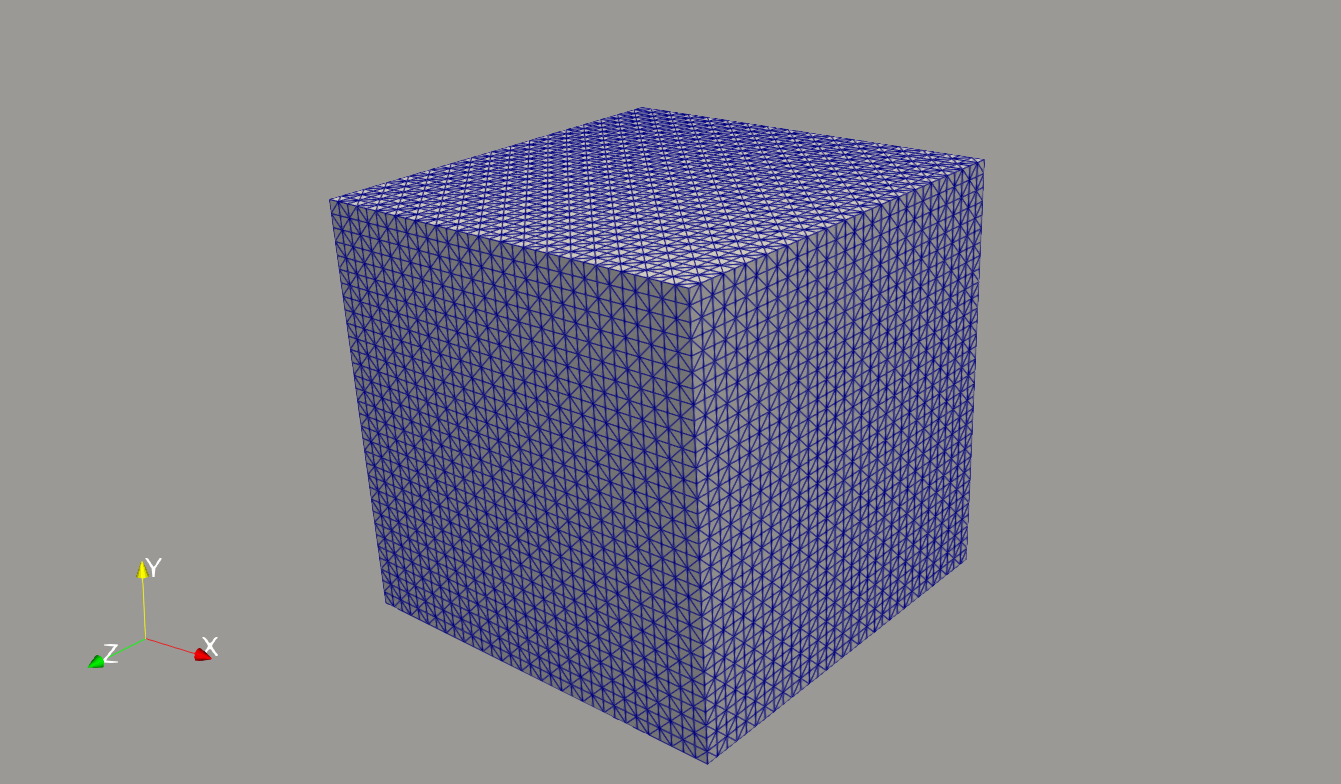
\includegraphics[width=\linewidth]{figures/mesh_cube.png}
    \caption{Mesh used for the simulation of a travelling planar wave in acoustic medium with \ac{ITM}}
    \label{fig:acoustic_mesh}
\end{figure}

We start our initial travelling wave at the origin and our wave travels to the boundary in $t = \frac{1}{2}$. We start our \ac{ITM} at $t=2$ such that the reversed wave will travel back to the origin at $t=4.0$ to meet the
forward going wave. 

\begin{figure}
    \centering
    \begin{subfigure}[b]{0.475\textwidth}
        \centering
        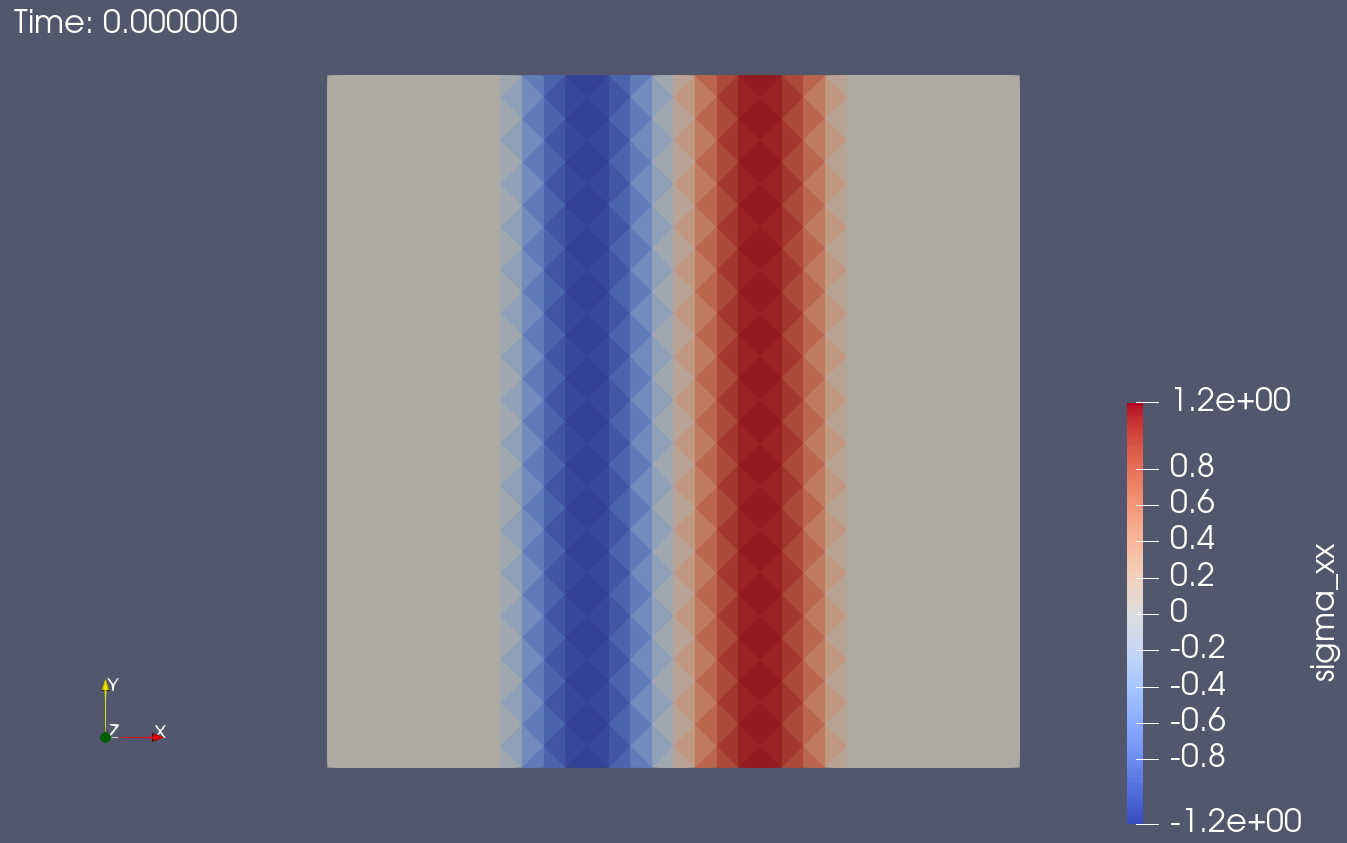
\includegraphics[width=\textwidth]{figures/travellingwave_t0.png}
        \caption{t=0} 
    \end{subfigure}
    \vskip\baselineskip
    \begin{subfigure}[b]{0.475\textwidth}   
        \centering 
        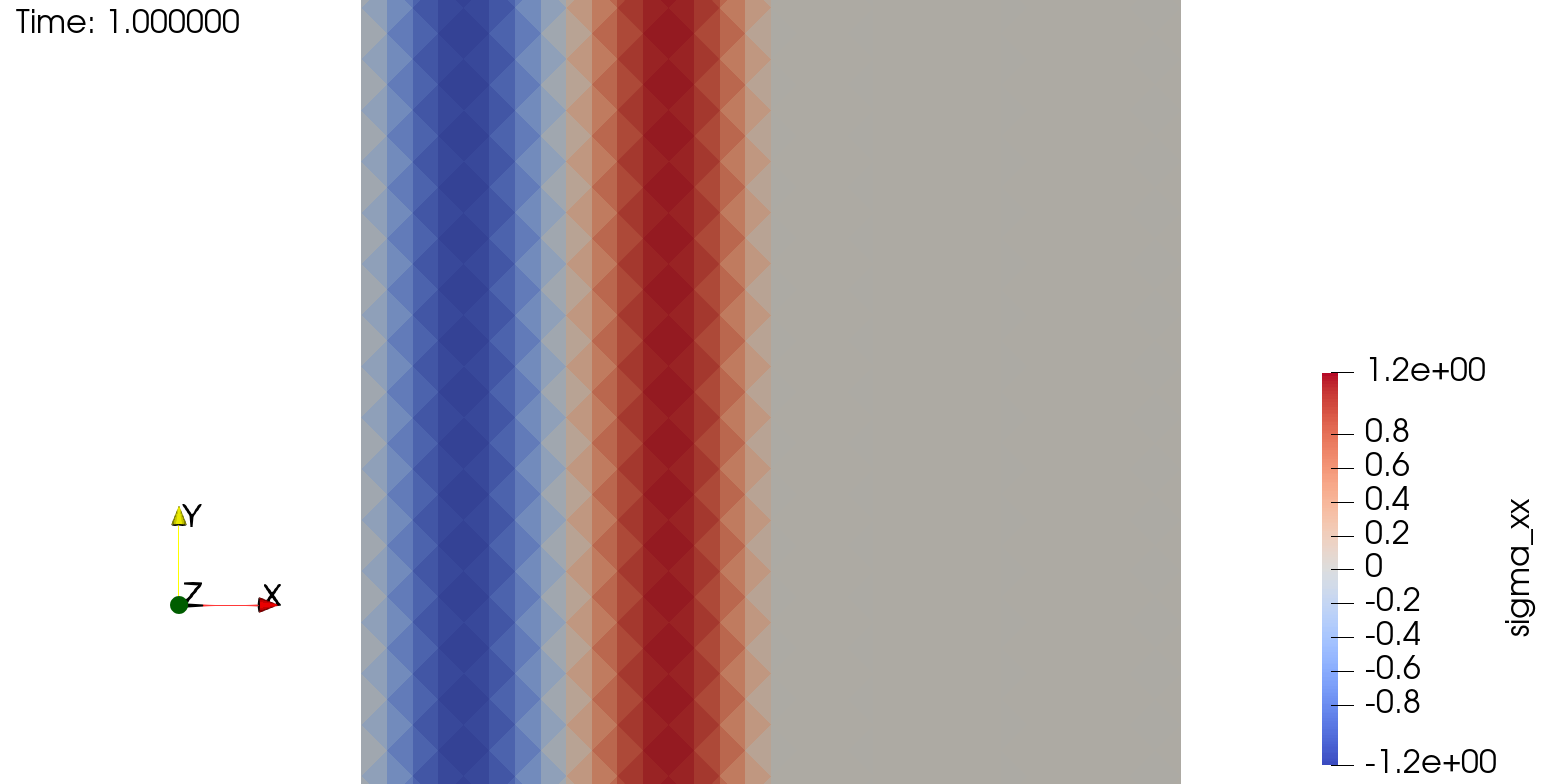
\includegraphics[width=\textwidth]{figures/travellingwave_t1.png}
        \caption{t=1.0}
    \end{subfigure}
    \hfill
    \begin{subfigure}[b]{0.475\textwidth}   
        \centering 
        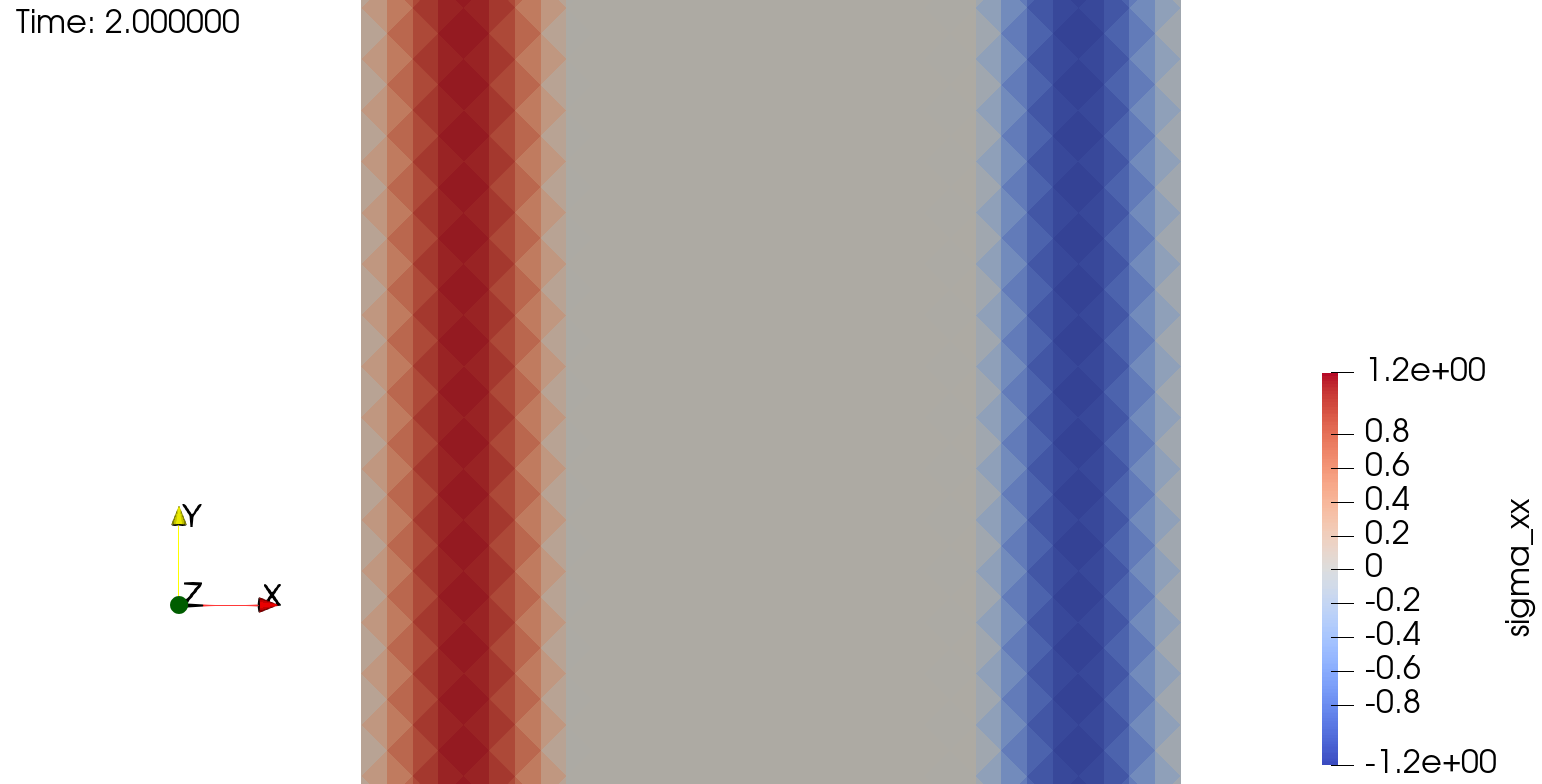
\includegraphics[width=\textwidth]{figures/travellingwave_t2.png}
        \caption{t=2.0}
    \end{subfigure}
    \vskip\baselineskip
    \begin{subfigure}[b]{0.475\textwidth}   
        \centering 
        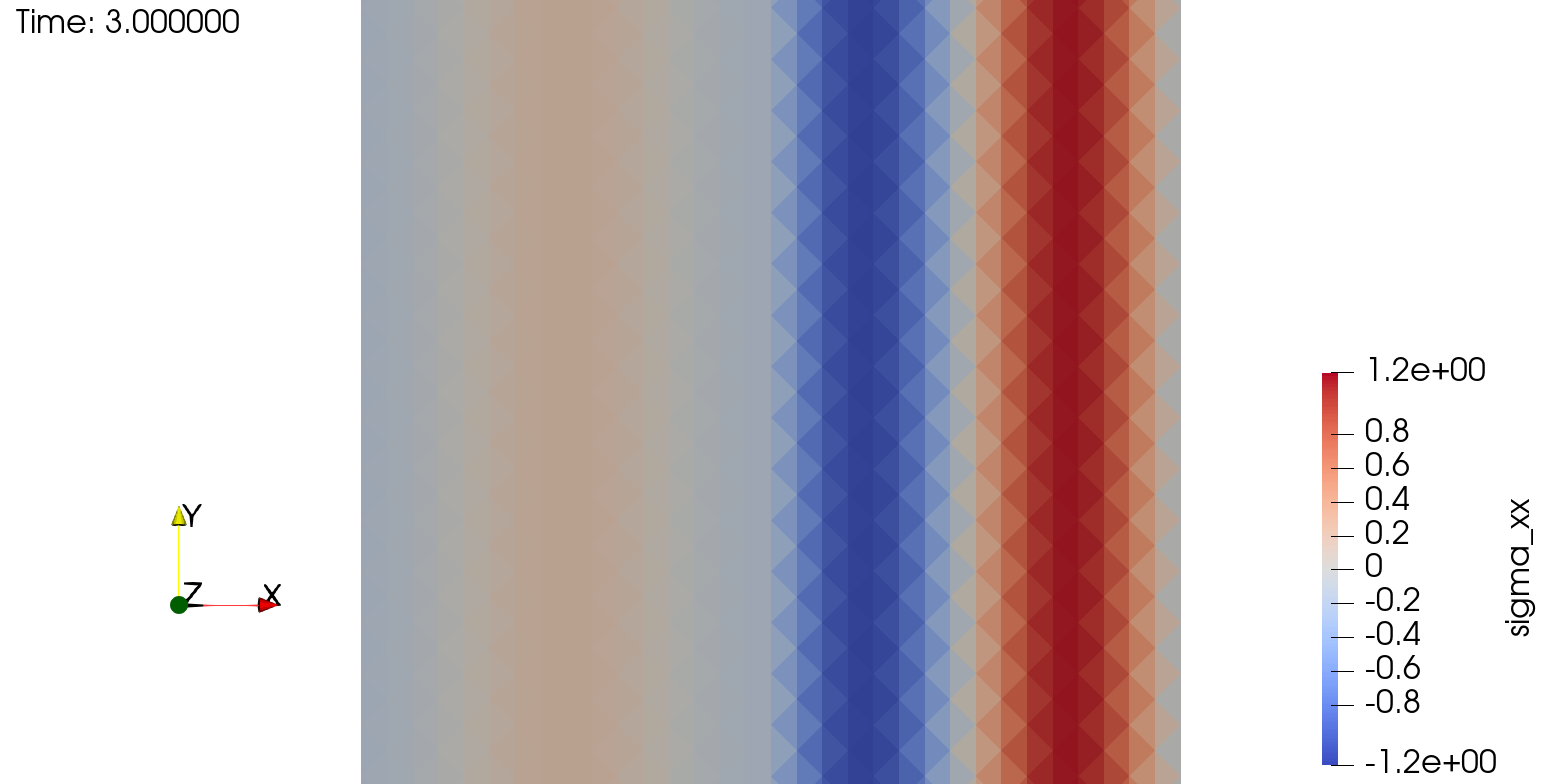
\includegraphics[width=\textwidth]{figures/travellingwave_t3.png}
        \caption{{t=3.0}}
    \end{subfigure}
    \hfill
    \begin{subfigure}[b]{0.475\textwidth}   
        \centering 
        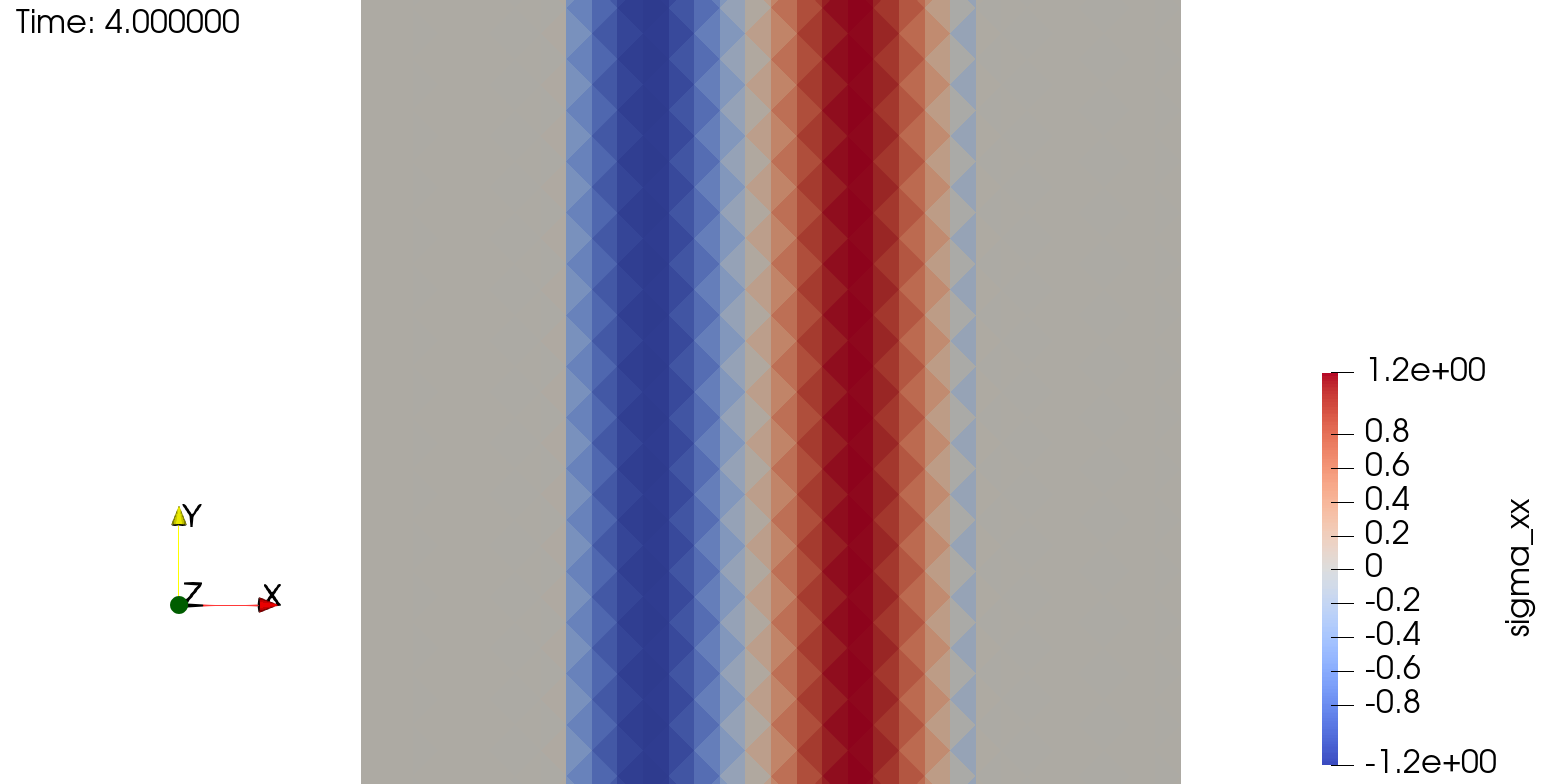
\includegraphics[width=\textwidth]{figures/travellingwave_t4.png}
        \caption{{t=4.0}}
    \end{subfigure}
    \caption{\ac{ITM} applied on a travelling planar wave in an acoustic media.}
\end{figure}

Here, we notice that there is a reflection of the forward going wave and it meets the the forward going wave at the origin at $t=4.0$. This is a proof of concept that the \ac{ITM} can be used to refocus waves in an acoustic media. \\

To observe the refocusing in a clearer way, we choose a slice perpendicular to the z-axis at $x=0$ and plot the wavefield in terms of u-velocity along the x-axis
at different times.We can see that at $t=2.0$, there is a reflected component along with the forward component. At $t=3.0$, i.e., half the time-period after
the application of the \ac{ITM}, we notice that the reflected component interacts with the forward wave for the first time. This shows that in half the time-period, the reflected wave travelled half the wave length interacting
with the forward travelling wave. At $t=4.0$, we notice that the reflected wave has travelled the entire wave length and is refocused at the origin. 
This is shown in figure \ref{fig:space-timeplot-travelling}.

\begin{figure}
    \centering
    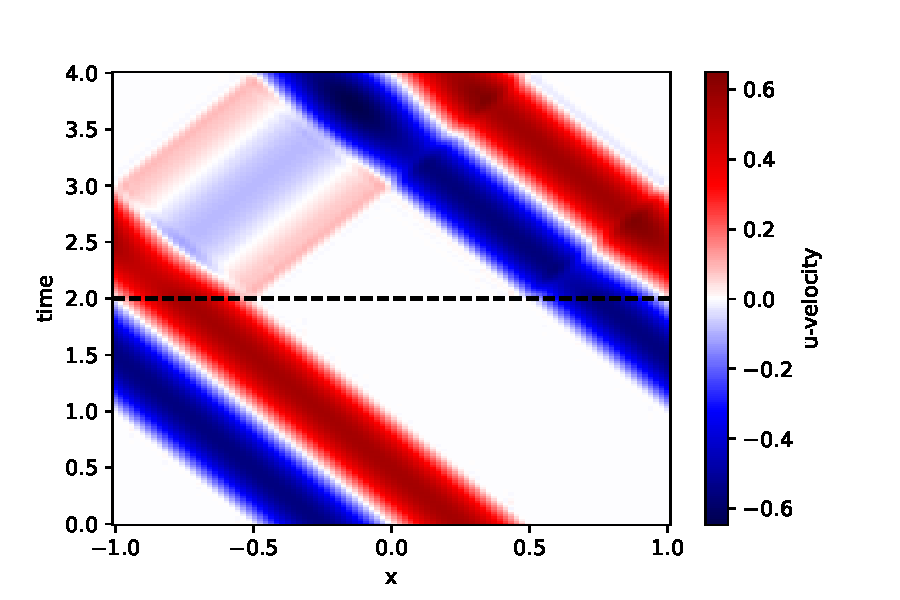
\includegraphics[width=0.75\linewidth]{figures/space-time-plot-travelling.pdf}
    \caption{Space Time plot for Acoustic Travelling Wave with \ac{ITM}. We take a slice perpendicular to the z-axis at $x=0$ and plot the u-velocity along the x-axis at different times.}
    \label{fig:space-timeplot-travelling}
\end{figure}

\section{Time-reversal of a velocity impulse point source in acoustic media} \label{sec:acousticITM}

We now consider a velocity impulse point source in an acoustic media. We pick the Lam\'{e} parameter $\lambda$, density $\rho$ 
from the half-space of the benchmark case WP2-LOH1~\footnote[1]{https://seissol.readthedocs.io/en/latest/pointsource.html} to make it a homogenous acoustic medium. 
The medium is characterized by the following parameters

\begin{align}
    \begin{split}
        \rho &=    2700.0 \\
        \mu &=     0.0 \\
        \lambda &= 3.24038016 \cdot 10^{10},
    \end{split}
\end{align}

This makes the velocity of the P-wave to be

\begin{equation}
    v_p = \sqrt{\frac{3.24038016 \cdot 10^{10}}{2700}} \approx 3464 .
\end{equation}

We choose a computational domain of [-26000,32000] X [-26000,32000] X [0,34000] and a simulation time of $t=10.0$ with \ac{ITM} applied at $t=5.0$ 
such that the originating waves do not reflect back from the boundaries at the x- and y-axis ensuring that
reflections due to \ac{ITM} are clearly noticeable. 
Our velocity impulse source is at [3000,3000,17000], the center of the domain. 
We have used an unstructured tetrahedral mesh with around 1.4 million elements. We have used more refinement in the region close to the source to capture the steep gradients as in figure \ref{fig:mesh-loh1}.

\begin{figure}
    \centering
    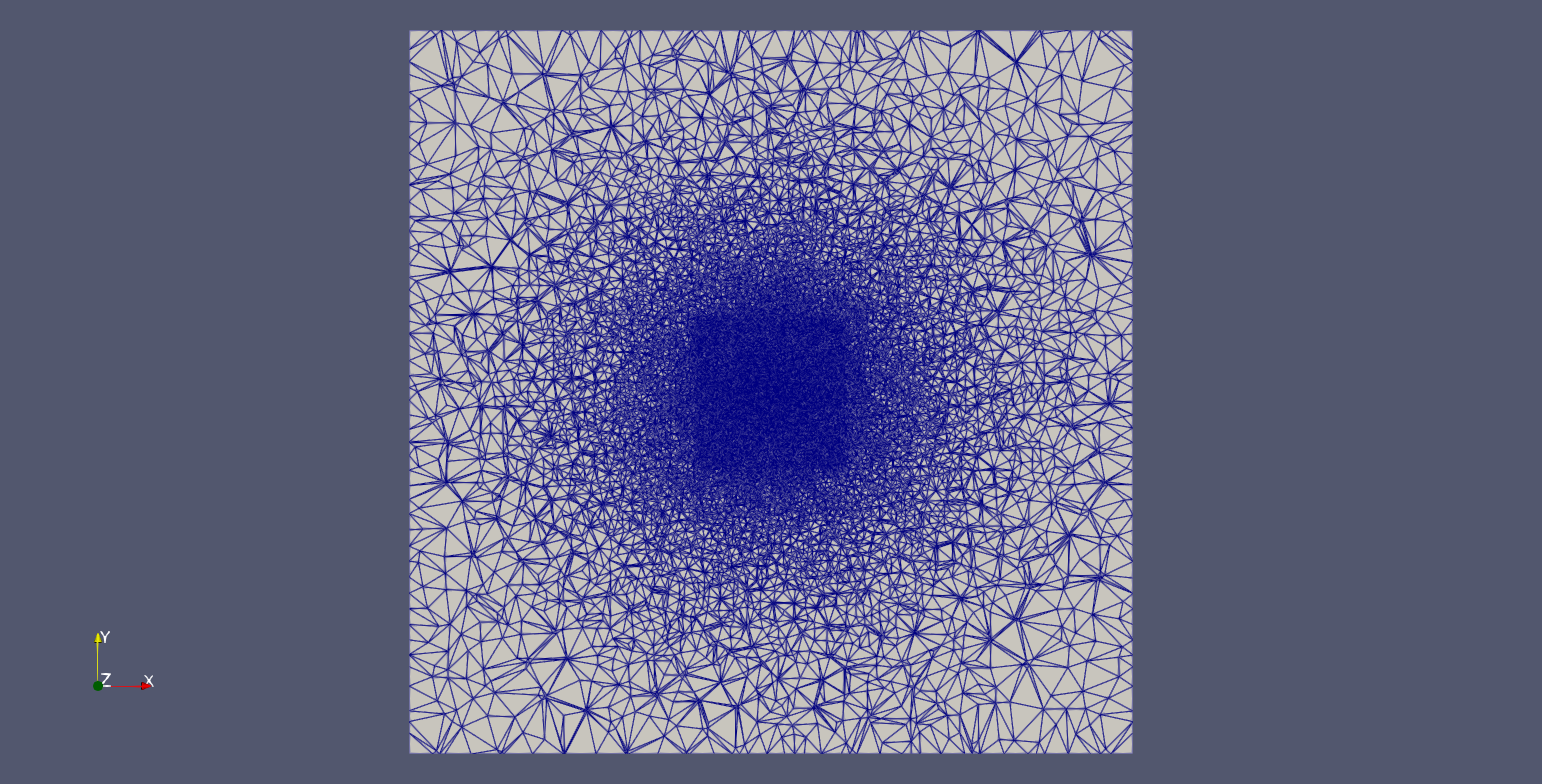
\includegraphics[width=\linewidth]{figures/mesh_loh1.png}
    \caption{Example mesh for simulations with a point source acting as a velocity pulse. We have a finer mesh near the source and a coarser mesh away from the source.}
    \label{fig:mesh-loh1}
\end{figure}

We apply a source as given in equation \ref{eq:source}. The source is then applied to equations 7 to 9 in equation \ref{eq:setofequations} as per the direction
$i$. $i=9$ is a velocity impulse point source in the Z-direction.

\begin{align}
    \begin{split}
        \dot{S} = \frac{1}{T^2} t e^{-\frac{t}{T}} \\
        S_i = \dot{S} \times C_i ,
    \end{split}
    \label{eq:source}
\end{align}

where T is a constant to decide the duration of the source approximately. We choose T=0.1. $i$ is the direction of the source. $i=7$ is a source applied in x-direction,
$i=8$ is a source applied in y-direction and $i=9$ is a source applied in z-direction. 
We choose the source to be in the Z-direction leads to $C_7 = 0, C_8 = 0, C_9 = 1.2 \cdot 10^{16}$. With this, our source looks like in figure \ref{fig:source}

\begin{figure}
    \centering
    \begin{tikzpicture}[scale=1.0]
        \begin{axis}[
            ylabel = $S_9$,
            xlabel = $t$]
            \addplot[domain=0:4, samples=1001, black, ultra thick]{1.2e16 * x*exp(-x/0.1)/(0.1*0.1)};
        \end{axis}
    \end{tikzpicture}
    \caption{Source term used for velocity impulse point source applied to z-velocity}
    \label{fig:source}
\end{figure}

We pick a slice at $Z=20000$, i.e., 3000 away from the source location in z-direction.
We visualise the wavefield with velocity in x-direction. With this setup and velocity impulse, we see that the velocity in x-direction
looks like in figure \ref{fig:space-timeplot-acousticnoITM}

\begin{figure}
    \centering
    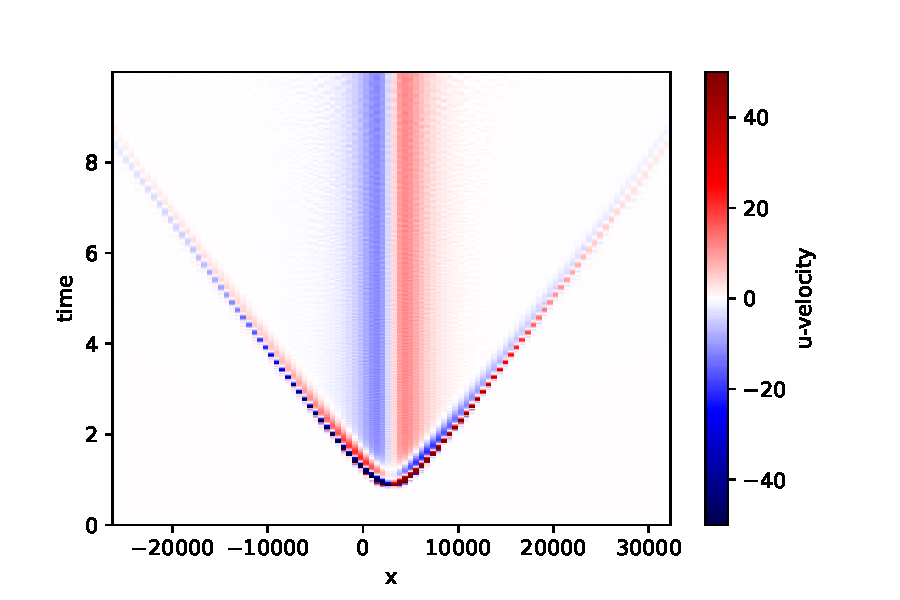
\includegraphics[width=0.75\linewidth]{figures/Acoustic-noITM.pdf}
    \caption{Space time plot for wave produced by velocity impulse point Source in acoustic Media. We take a slice at $Z=20000$ perpendicular to z-axis 
    and plot the u-velocity along x-axis at different times.}
    \label{fig:space-timeplot-acousticnoITM}
\end{figure}

We notice that we have only one wave propagating in time as expected as we have an acoustic media and it reaches our slice around 1.5 seconds. 
We have observed an unexpected stationary velocity in the vicinity of the source, which requires a thorough investigation by means of SeisSol. But it does not affect our refocusing and has nothing to do with
our application of \ac{ITM}. We now apply ITM on the same setup at $t=5.0$. We notice that the wavefield looks like in figure \ref{fig:space-timeplot-acousticITM}

\begin{figure}
\begin{subfigure}[t]{0.49\textwidth}   
    \centering 
    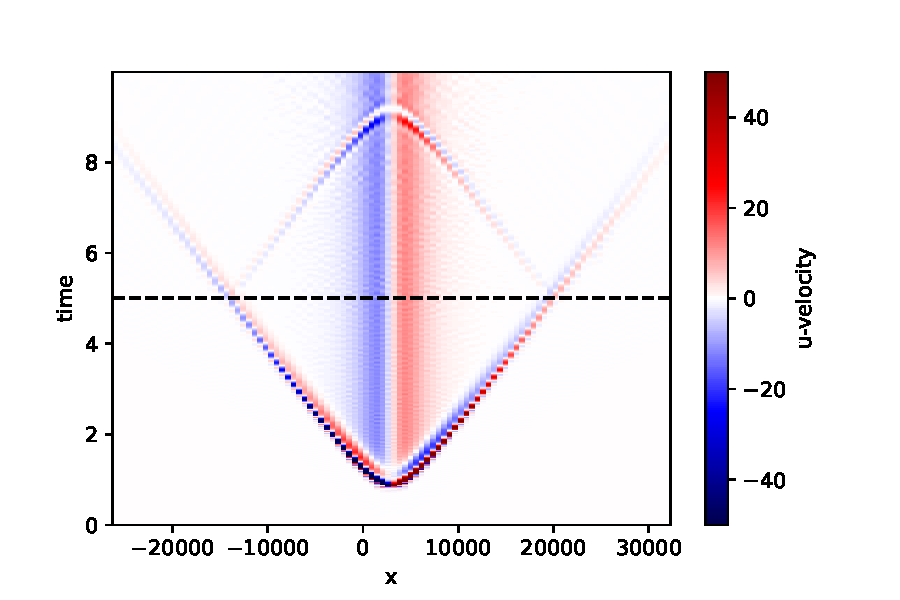
\includegraphics[width=\textwidth]{figures/AcousticITM.pdf}
    \caption{Wave produced by velocity impulse in acoustic media with \ac{ITM}}
\end{subfigure}
\hfill
\begin{subfigure}[t]{0.49\textwidth}   
    \centering 
    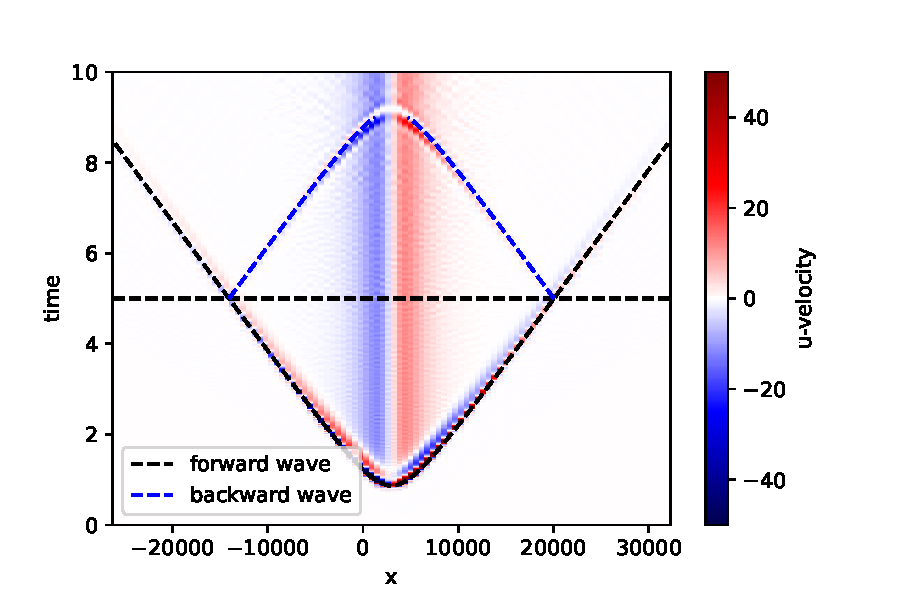
\includegraphics[width=\textwidth]{figures/AcousticITMAnnotated.pdf}
    \caption{Expected location of forward and reflected waves in time. The dashed lines denote the expected location of the wavefronts at given time.}
    \label{subfig:acousticITMAnnotated}
\end{subfigure}
\caption{Space time plot for wave produced by velocity impulse point source in acoustic media with \ac{ITM}. We take a slice at $Z=20000$ perpendicular to z-axis
and plot the u-velocity along x-axis at different times.}
\label{fig:space-timeplot-acousticITM}
\end{figure}

We notice that there is a reflected wave travelling back to the source. We notice that the reflected wave leaves our slice around $t=8.5$, showing that the reflected wave
is reflected along the line $t=5.0$, which is our point in time when we applied the \ac{ITM}. In figure \ref{fig:space-timeplot-acousticITM}, we plot the expected
location of the wave front from the forward going and reflected waves assuming spherical waves being generated at the source and that the reflected wave is spherical
and has the same speed as the original incident wave in figure \ref{subfig:acousticITMAnnotated}. This confirms that the application of \ac{ITM} produces a reflected wave
successfully in Acoustic Media. \\

\section{Time-reversal of a velocity impulse point source in an elastic media} \label{sec:elasticITM}
We now consider a velocity impulse point source like in Section \ref{sec:acousticITM}. We choose the material parameters from the half-space of the 
benchmark case WP2-LOH1~\footnote[1]{https://seissol.readthedocs.io/en/latest/pointsource.html} to make it a homogenous elastic medium. The material parameters 
are characterized by

\begin{align}
    \begin{split}
        \rho &=    2700.0 \\
        \mu &=     3.23980992 \cdot 10^{10} \\
        \lambda &= 3.24038016 \cdot 10^{10} ,
    \end{split}
\end{align}

which makes the velocities of P- and S-waves to be

\begin{align}
    \begin{split}
        v_p &= 6000.0 \\
        v_s &= 3464.0 .
    \end{split}
\end{align}

In this case we extend our computational domain even further to [-104000,128000] X [-104000,128000] X [0,136000] and a simulation time of $t=18.0$ with \ac{ITM} applied at $t=9.0$
such that the originating waves do not reflect back from the boundaries at the x- and y-axis ensuring that reflections due to the \ac{ITM} are clearly noticeable.
Our velocity impulse source is at [12000,12000,68000] such that it is exactly at the center of the domain.
We chose to analyse the simulation for a longer time in this scenario such that the S-wave reaches the slice. We choose an unstructured tetrahedral mesh with around 13 million elements similar to the acoustic case. 
We apply a source which has already been discussed in equation \ref{eq:source} and figure \ref{fig:source}. \\

We pick a slice at $Z = 40000$ and visualise the wavefield with velocity in x-direction and the displacement along the x-axis. With this setup and velocity impulse, 
we see that the velocity in x-direction looks like in figure \ref{fig:space-timeplot-elasticnoITM}.

\begin{figure}
    \centering
    \includegraphics[width=0.75\linewidth]{figures/noITMElasticvelocity.pdf}
    \caption{Space time plot for waves produced by velocity impulse point source in elastic media. We take a slice at $Z=40000$ perpendicular to z-axis
    and plot the u-velocity along x-axis at different times.}
    \label{fig:space-timeplot-elasticnoITM}
\end{figure}

We integrate the obtained velocity field to plot displacement field in X- direction as shown in figure \ref{fig:space-timeplot-elasticnoITMdisplacement}.

\begin{figure}
    \centering
    \includegraphics[width=0.75\linewidth]{figures/noITMElasticdisplacement.pdf}
    \caption{Space time plot for waves produced by velocity impulse point source in elastic media. We take a slice at $Z=40000$ perpendicular to z-axis
    and plot the displacement in x-direction along x-axis at different times. We integrate the velocity field to obtain the displacement field.}
    \label{fig:space-timeplot-elasticnoITMdisplacement}
\end{figure}

We can clearly notice two propagating waves as expected as we are dealing with an elastic media now. We notice a static displacement field in between the two waves.
This is a common phenomenon in displacement fields built with simulation codes in seismic simulations(cite?). 
We now apply \ac{ITM} on the same setup at $t=9.0$. We notice that the wavefield looks like in figure \ref{fig:space-timeplot-elasticITM}

\begin{figure}
    \centering
    \includegraphics[width=0.75\linewidth]{figures/Elastic-tworeflections.pdf}
    \caption{Space time plot for waves produced by velocity impulse point source in elastic media with \ac{ITM}. We take a slice at $Z=40000$ perpendicular to z-axis
    and plot the u-velocity along x-axis at different times.}
    \label{fig:space-timeplot-elasticITM}
\end{figure}

We notice that there are two clearly reflected waves travelling back to the source. We notice that the faster moving wave i.e., P-wave leaves our slice around 
$t=13.0$ which is around 4 seconds after the application of \ac{ITM} which is the time it travelled through the slice just before the application of \ac{ITM}. 
We notice that the slower moving wave, i.e., S-wave also has a reflection symmetric about line $t=9.0$. We now plot the displacement plot in x-direction on the 
slice just like we did in figure \ref{fig:space-timeplot-elasticnoITMdisplacement} in \ref{fig:space-timeplot-elasticITMdisplacement}.

\begin{figure}
    \centering
    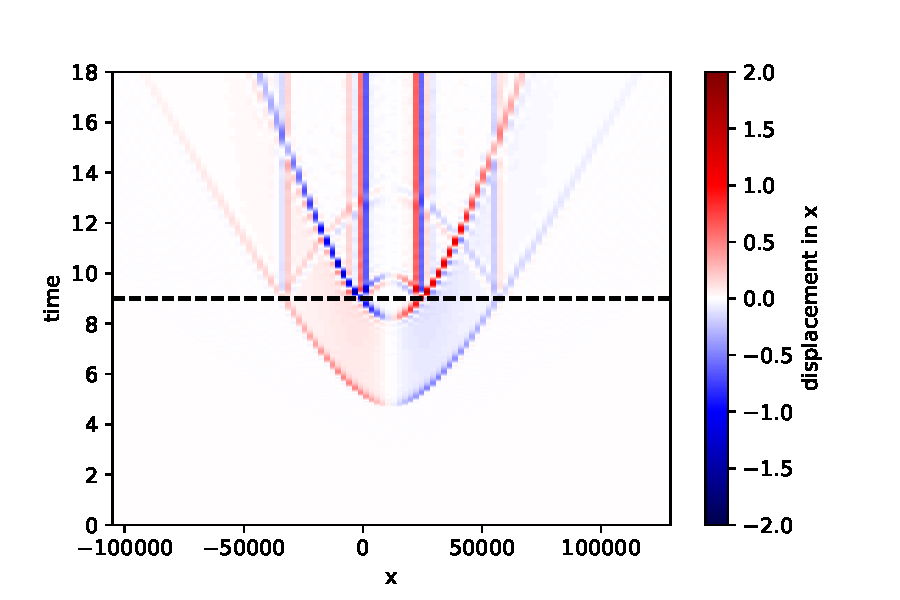
\includegraphics[width=0.75\linewidth]{figures/Elastic-tworeflections-displacement.pdf}
    \caption{Space time plot for waves produced by velocity impulse point source in elastic media with \ac{ITM}. We take a slice at $Z=40000$ perpendicular to z-axis
    and plot the displacement in x-direction along x-axis at different times. We integrate the velocity field to obtain the displacement field.}
    \label{fig:space-timeplot-elasticITMdisplacement}
\end{figure}

We can clearly see two reflections even in case of the displacement wave field too and the static displacements between the two waves persist. But we see extra features
here in case of the displacement wave-field. We obtain extra static displacements in time as vertical streaks which originate from the point where the waves meet the slice
at \ac{ITM}. These are not yet explained but we suspect they may be explained either by the physical phemonenon or due to the numerical implementation or due to errors
produced to numerical integration of the velocity wavefields. \\

This shows that both the waves can be reflected simultaneously by scaling the material parameters to change their impedance to obtain a component which 
is reflected back to its source. \\

\section{Time-reversal of P- wave of a velocity impulse point source in elastic media} \label{sec:elasticITMpwave}
We now demonstrate the reflection of just the P- wave by scaling the Lam\'{e} parameter $\lambda$ and keeping the second Lam\'{e} parameter $\mu$ constant.\\
The same setup is used as in Section \ref{sec:elasticITM} and we try to reflect just the P- wave while letting the S- wave travel unaffected in time. The slice
and everything else about the simulation remain the same. The wavefields without \ac{ITM} looks like in figures \ref{fig:space-timeplot-elasticnoITM} and
\ref{fig:space-timeplot-elasticnoITMdisplacement}

\begin{figure}
    \centering
    \includegraphics[width=0.75\linewidth]{figures/pwave-ITM1.pdf}
    \caption{Reflection of P-wave in elastic Media with \ac{ITM}. We take a slice at $Z=40000$ perpendicular to z-axis
    and plot the u-velocity along x-axis at different times.}
    \label{fig:space-timeplot-pwave}
\end{figure}

After the application of the \ac{ITM}, we see reflections in the wavefield in figure \ref{fig:space-timeplot-pwave}.
As the reflection in figure \ref{fig:space-timeplot-pwave} is seen but is faint. We plot the same with a different colorbar just to show the reflection in a clearer
way in figure \ref{fig:space-timeplot-pwave2}

\begin{figure} %% replace pictures. Not clear and being cut
    \centering
    \includegraphics[width=0.75\linewidth]{figures/pwave-ITM2.pdf}
    \caption{Reflection of P-wave in elastic media with \ac{ITM}. We take a slice at $Z=40000$ perpendicular to z-axis
    and plot the u-velocity along x-axis at different times. We use a different colorbar from figure \ref{fig:space-timeplot-pwave} to show the reflection more clearly.}
    \label{fig:space-timeplot-pwave2}
\end{figure}

We can clearly see here in this plot that there is a P- wave which is reflected without affecting the S- wave. This provides us a proof of concept where we 
can reflect one wave by changing its impedance while maintaining the other wave's impedance constant. \\

\begin{figure} %% replace pictures. Not clear and being cut
    \centering
    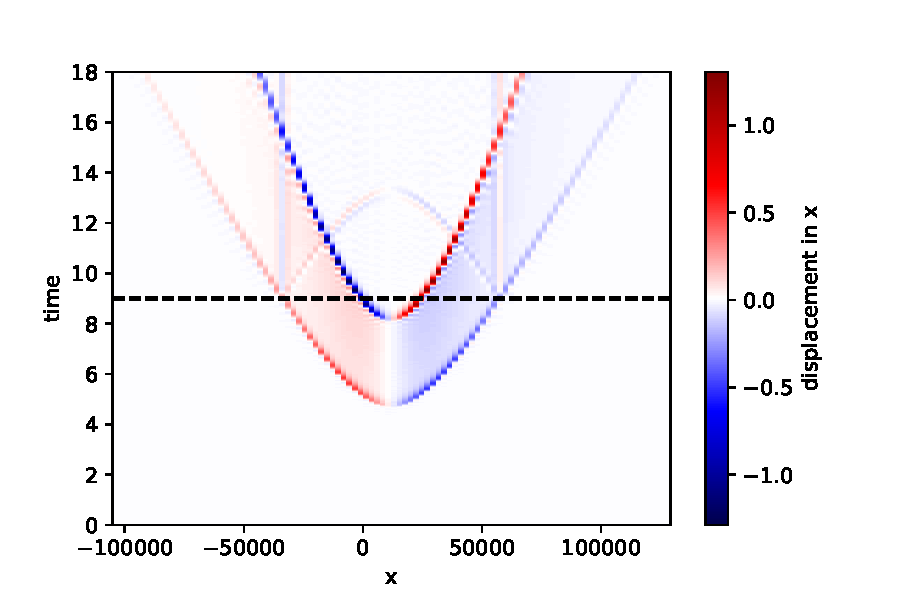
\includegraphics[width=0.75\linewidth]{figures/pwave-ITMdisplacement.pdf}
    \caption{Reflection of P-wave in Elastic Media with \ac{ITM}. We take a slice at $Z=40000$ perpendicular to z-axis
    and plot the displacement in x-direction along x-axis at different times. We integrate the velocity field to obtain the displacement field.}
    \label{fig:space-timeplot-pwavedisplacement}
\end{figure}

We plot the displacement wavefield in figure \ref{fig:space-timeplot-pwavedisplacement} and we can see the reflected P- wave in displacement wavefield and the static
displacement is noticed in this case too just like in the case of reflecting both the waves. 

\section{Time-reversal of S-wave of a velocity impulse point source in elastic media} \label{sec:elasticITMswave}
In this section, we demonstrate the reflection of just the S- wave by modifying the Lam\'{e} parameters such that P-wave does not
get reflected but the S- wave does. The same setup is used as in section \ref{sec:elasticITM}. The wavefields without \ac{ITM} looks like in figures in \ref{fig:space-timeplot-elasticnoITM}
and \ref{fig:space-timeplot-elasticnoITMdisplacement}. \\

After the application of the \ac{ITM}, we see reflections in the wavefield in figure \ref{fig:space-timeplot-swave} showing the zoomed version near the 
\ac{ITM} so that the reflected part is clearly visible in subfigure \ref{subfig:swavezoomed}.

\begin{figure}
    \begin{subfigure}[t]{0.49\textwidth}   
        \centering 
        \includegraphics[width=\textwidth]{figures/swaveITM1.pdf}
        \caption{Reflecting S-wave in elastic media. We take a slice at $Z=40000$ perpendicular to z-axis
        and plot u-velocity along x-axis at different times.}
        \label{subfig:swave}
    \end{subfigure}
    \hfill
    \begin{subfigure}[t]{0.49\textwidth}   
        \centering 
        \includegraphics[width=\textwidth]{figures/swaveITM2.pdf}
        \caption{Zoomed cut section of figure \ref{subfig:swave} to show the reflected S-wave more clearly.}
        \label{subfig:swavezoomed}
    \end{subfigure}
    \caption{Reflection of S-wave in elastic media with \ac{ITM}. We take a slice at $Z=40000$ perpendicular to z-axis and plot u-velocity along x-axis at different times.}
    \label{fig:space-timeplot-swave}
\end{figure}
    
We plot the displacement wavefield in figure \ref{fig:space-timeplot-swavedisplacement} and we can see the reflected S- wave in displacement 
wavefield and the static displacement like in previous section persists. We need more investigation into this to make sense of this static displacement.

\begin{figure}
    \centering
    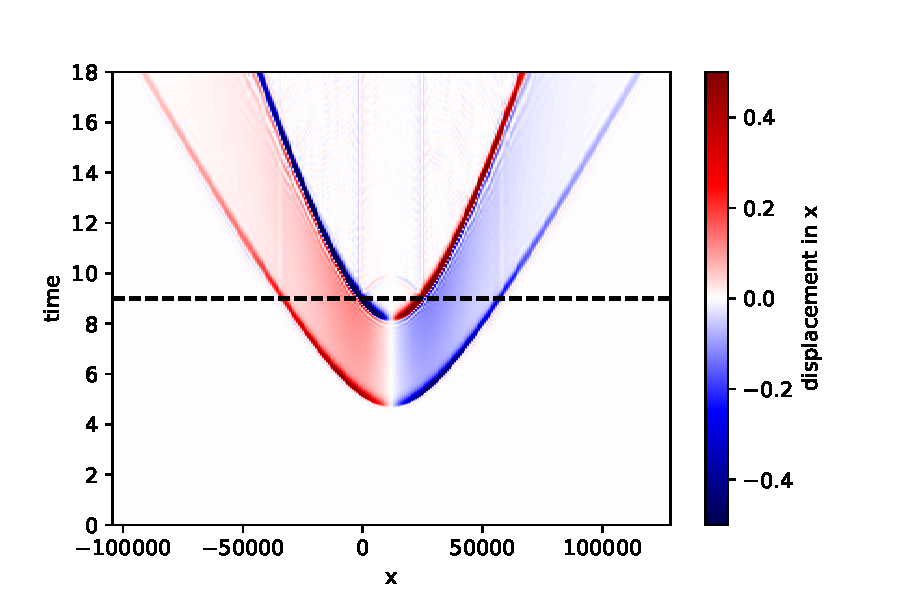
\includegraphics[width=0.75\linewidth]{figures/swaveITMdisplacement.pdf}
    \caption{Reflection of S-wave in elastic media with \ac{ITM}. We take a slice at $Z=40000$ perpendicular to z-axis
    and plot the displacement in x-direction along x-axis at different times. We integrate the velocity field to obtain the displacement field.}
    \label{fig:space-timeplot-swavedisplacement}
\end{figure}

We can clearly see here in this plot that there is a S- wave which is reflected without affecting the P- wave. 
This provides us a proof of concept where we show that we can reflect one wave by changing its impedance while maintaining the other wave's impedance constant. \\

\section{Time-reversal of a pressure impulse point source in acoustic media}
We choose the same material and mesh as in section \ref{sec:acousticITM} and change the source term to a pressure impulse. A pressure impulse source term is a moment tensor
with all non-diagonal elements zero and equal non-zero diagonal elements. These are applied to the first three equations of the set of equations \ref{eq:setofequations}. 
An exponentially decaying source is chosen similar to the source in section \ref{sec:acousticITM}. With this setup, the normal propagation of the wave looks at a slice which is already explained in section \ref{sec:acousticITM}
like in figure \ref{fig:space-timeplot-pressurenoITM}.

\begin{figure}
    \centering
    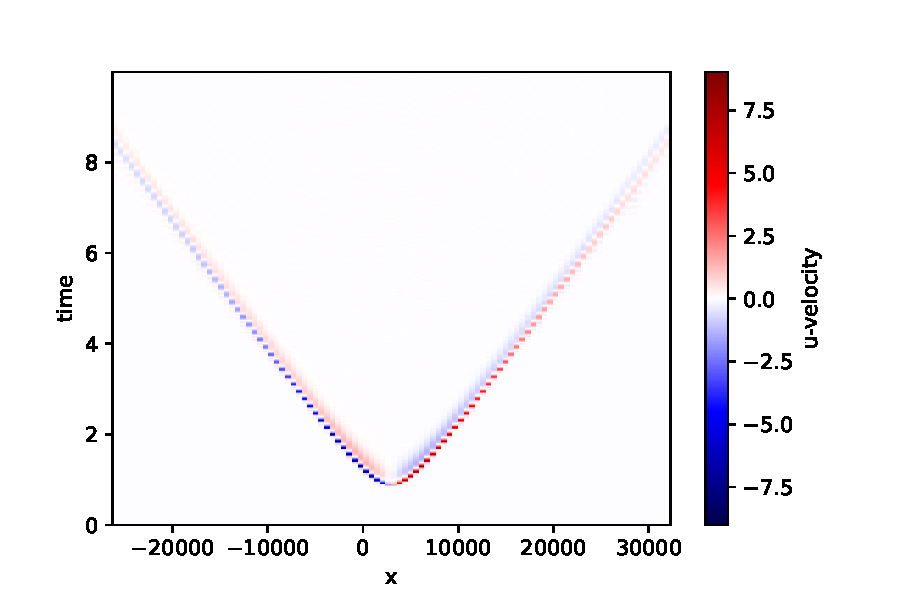
\includegraphics[width=0.75\linewidth]{figures/pressureimpulsewave-noITM.pdf}
    \caption{Pressure impulse in acoustic media}
    \label{fig:space-timeplot-pressurenoITM}
\end{figure}

\section{Convergence Test}\label{sec:convergence}
We now perform a convergence test to verify that our \ac{ITM} implementation is accurate and converges with our \ac{ADER}-\ac{DG} scheme. 
We check the error between our numerical implementation and the analytical solution developed in section \ref{section:3DITMAcoustic}. 
The mesh is setup with equal triangular elements on a cubic domain of [-1, 1] X [-1, 1] X [-1, 1] with the number of elements in each direction varying in [4, 8, 16, 32, 64, 128].
We calculate the $L^2$ error of the solution with respect to the analytical solution as per section \ref{section:3DITMAcoustic}. We calculate this error for different polynomial
orders within [1, 2, 3, 4, 5] used in the reference element of the \ac{DG} scheme. We expect a convergence order of $p+1$ where $p$ is the polynomial order used in the
\ac{DG} scheme used ~\parencite{cockburn2011discontinuous}. We mow plot the $L^2$ error norm of $u$- velocity in figure \ref{fig:convergence}.

\begin{figure}
    \centering
    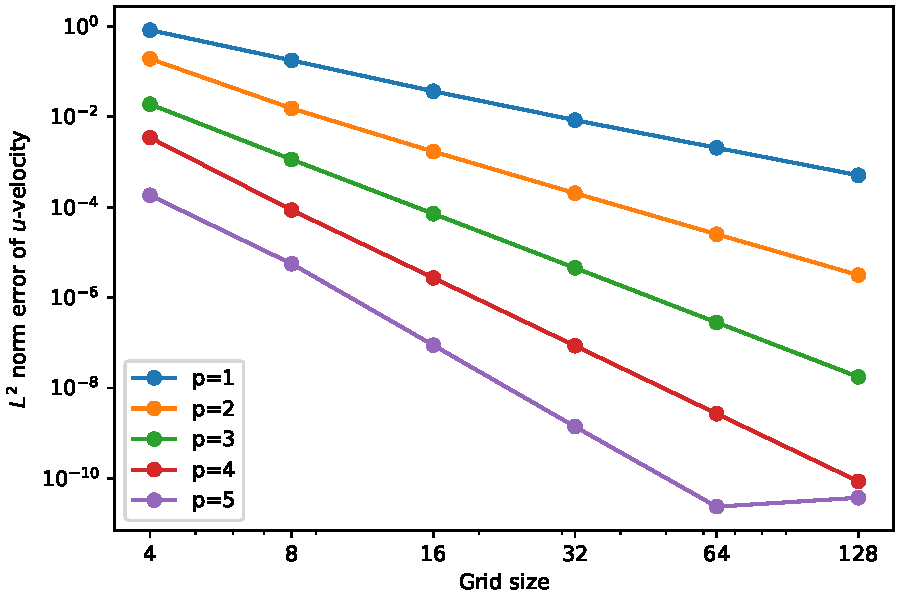
\includegraphics[width=0.75\linewidth]{figures/error1.pdf}
    \caption{Convergence plot for $L^2$ norm of $u$-velocity for acoustic travelling wave with \ac{ITM}. The error is calculated with respect to the analytical solution
    in section \ref{section:3DITMAcoustic}.}
    \label{fig:convergence}
\end{figure}

We notice that the slope of the curve increases as expected with increasing order of the polynomial. In case of order 5, we notice that there is a slight increase
of error for grid size 128. This is suspected due to the error plateauing as the precision hits the floating point precision. We perform a linear fit on the log-log
plot to get a slope such that we can check the convergence order of the plot. We remove the last point from the fit for $p=5$ as it is suspected to be an outlier. 
We get the following convergence orders for different polynomial orders shown in table \ref{table:convergenceorder} and figure \ref{fig:convergenceorder}.

\begin{center}
\begin{table}[]
    \centering
    \caption{Convergence order vs polynomial order obtained from the convergence study of acoustic travelling wave with \ac{ITM}}.
    \label{table:convergenceorder}
    \begin{tabular}{|l|l|}
        \hline
     \textbf{Polynomial Order}& \textbf{Convergence Order}  \\
     \hline
     1 & 2.13\\
     \hline
     2 & 3.15 \\
     \hline
     3 & 4.00 \\
     \hline
     4 & 5.03 \\
        \hline
        5 & 5.77\\
        \hline
    \end{tabular}
    \end{table}
\end{center}

\begin{figure}
    \centering
    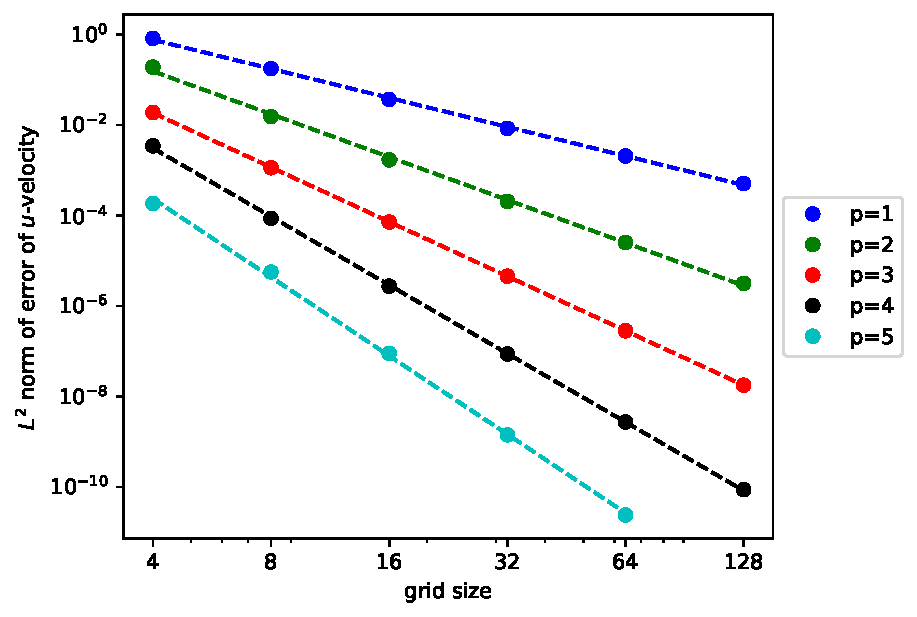
\includegraphics[width=\linewidth]{figures/error2.pdf}
    \caption{Linear fit of $\log\left(L^2\right)$ and $\log\left(grid size\right)$  plot for acoustic travelling wave with \ac{ITM}. The slope of the dashed lines denote the 
    obtained convergence order.The outlier for $p=5$ is removed from the fit.}
    \label{fig:convergenceorder}
\end{figure}

We now plot the expected error with the expected convergence order vs the actual error during the simulations in figure \ref{fig:expectedvsactualerror}.

\begin{figure}
    \centering
    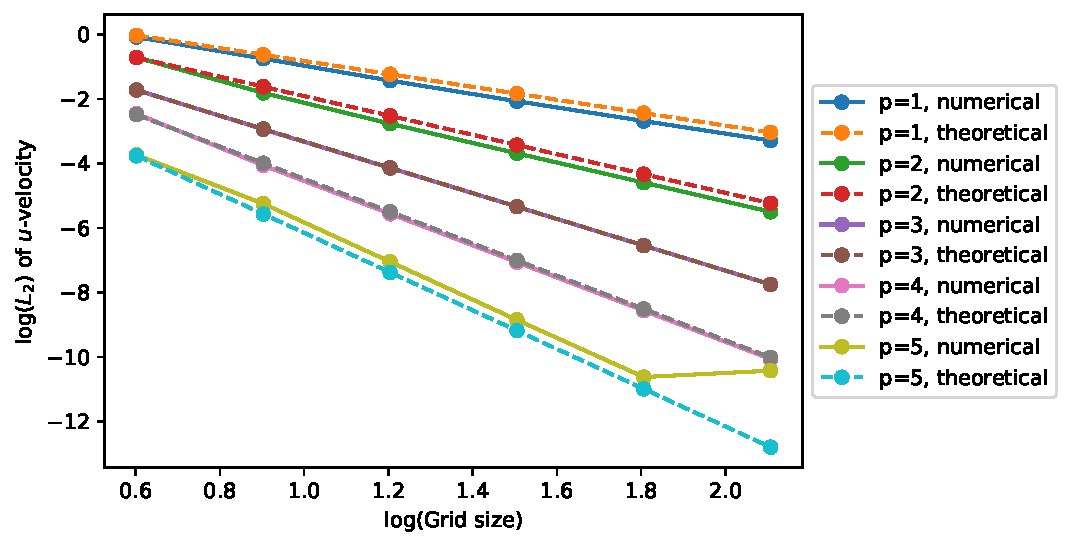
\includegraphics[width=\linewidth]{figures/error3.pdf}
    \caption{Expected $L^2$ norm vs actual $L^2$ norm for acoustic travelling wave with \ac{ITM}. The expected error is calculated with the expected convergence order
    as the slope and the mean of logarithms of errors as the intercept of the line.}
    \label{fig:expectedvsactualerror}
\end{figure}

\section{Discussion}
In this chapter, we looked at the results obtained from applying the \ac{ITM} on seismic waves. We began with the reflection of a travelling planar wave in acoustic media
and then moved on to a spherical waves generated by a velocity impulse point source in acoustic and elastic media. 
We then looked at the reflection of just the P- wave and S- wave separately to show that we can reflect just one wave by changing its impedance while keeping the other wave's impedance constant.
In the end, we ran a convergence study of our implementation with the analytical solution obtain in section \ref{section:3DITMAcoustic} to conclude that our implementation
is convergent with the expected convergence order. \\

\chapter{Conclusion and Future Research Outlook}\label{chapter:Conclusion}
In this thesis, we implemented and analysed the wavefield reversal method \ac{ITM} in the numerical simulation software SeisSol. We first presented the basic theory of elastic wave propagation and the numerical \ac{ADER}-\ac{DG} scheme used in SeisSol in chapter \ref{chapter:seismicwaves}.
We then presented the theoretical foundation of the \ac{ITM} method in chapter \ref{chapter:TimeReversal}, the expected solutions for a simple one dimensional case in section \ref{section:ITMAcoustic} and the wavefield reversal for a three dimensional wave in acoustic medium in section \ref{section:3DITMAcoustic}.
The energy behaviour of the \ac{ITM} method was analysed for different phases of the \ac{ITM}.
We then presented the implementation details of the \ac{ITM} method in SeisSol in section \ref{section:Implementation}. The implementation details 
for different wave reversal scenarios were discussed in sections \ref{sec:reflecting_both}, \ref{sec:reflecting_both_constant}, \ref{sec:reflecting_p}, \ref{sec:reflecting_s} and the required modifications for the time step size were discussed in section \ref{sec:time_step_size}. \\

Finally, we presented the results of various studies conducted to analyse the effects of different scenarios on the wavefield reversal in chapter \ref{chapter:Results}.
We first reverse a planar acoustic wave in a homogeneous medium in section \ref{sec:acoustictravelling} and analyse the reversal to verify that the reversed and forward waves have identical speeds as expected from the analytical soutions.
We later reverse spherical waves generated by point sources in WP2-LOH1 case, modified to make the medium homogeneous, in acoustic and elastic media in sections \ref{sec:acousticITM} and \ref{sec:elasticITM}. We verify that the reversal of just one wave is possible while letting 
the other wave stay forward propagating in sections \ref{sec:elasticITMpwave} and \ref{sec:elasticITMswave}. We then verify that our implementation in SeisSol is converging by verifying the numerical results with the analytical solutions developed is increased in section \ref{sec:convergence}. We notice that
the numerical results are converging faster to the analytical solutions as the polynomial order of the \ac{DG} scheme increases. This verifies that the \ac{ITM}
method proposed by ~\parencite{Bacot2016} on waterwaves can be applied analogously on seismic waves to obtain a reversed component retracing them to the source. \\

Currently, the \ac{ITM} parameters are heuristically determined. As part of future research, analytical solutions for the spherical waves produced by point sources may be calculated to select the appropriate parameters for \ac{ITM}. More complex scenarios and wavefield reversal in heterogeneous media can be studied. 
The \ac{ITM} method may be used to study the effects of different wave propagation properties on the wavefield reversal. \ac{ITM} approach and its implementation 
for other scenarios like anisotropic, viscoelastic and poroelastic media can be studied. Noise in the simulation data obtained during the reversal process
could be filtered out to obtain a clearer refocusing pattern and more accurate analysis in the phase shift could be performed.\\
% TODO: add more chapters here

\appendix{}

\microtypesetup{protrusion=false}

\addchap{Abbreviations}
\begin{acronym}
	\itemsep-.25\baselineskip
	\acro{TUM}[TUM]{Technical University of Munich}
	\acro{TRM}[TRM]{Time-reversal Mirror}
	\acro{ITM}[ITM]{Instantaneous Time Mirror}
	\acro{DG}[DG]{Discontinuous Galerkin}
	\acro{ADER}[ADER]{Arbitrary high-order schemes using DERivates}
	\acro{DG-FE}[DG-FE]{Discontinuous Galerkin Finite Element}
	\acro{RK-DG}[RK-DG]{Runge Kutta Discontinuous Galerkin}
	\acro{CFL}[CFL]{Courant-Friedrichs-Lewy}
	\acro{LTS}[LTS]{Local Time Stepping}
	% TODO: add acronyms
\end{acronym}

\listoffigures{}
\listoftables{}
\microtypesetup{protrusion=true}
\printbibliography{}

\end{document}
